%=======================================================================
%  Thermal analysis of a power-to-heat-to-power system with cascaded
%  latent heat storage in repurposed oil and gas wells.
%
%  Elsevier elsarticle class (preprint layout).
%  Structure follows the IHTC-18 paper (Ko & Barbosa, "Thermal analysis of
%  a power-to-heat-to-power system using repurposed oil wells for energy
%  storage"); the model content follows P2H2P_model.ipynb, model v0.13
%  (isentropic efficiencies on the state points; exergy audit with the
%  geothermal source priced under the 'resource' convention).
%
%  Files:
%     P2H2P_main.tex            this file (front matter, packages, macros)
%     p2h2p_intro.tex           1  Introduction
%     p2h2p_model.tex           2  Modelling (2.1-2.5)
%     p2h2p_exergy.tex          2.6 Exergy analysis
%     p2h2p_implementation.tex  3  Mathematical implementation
%     p2h2p_results.tex         4  Results (skeleton) and 5 Conclusions
%     p2h2p_refs.bib            bibliography
%  Figures reused from the IHTC-18 project (upload to this project to
%  replace the placeholder frames):
%     Block_diag_ch.png, Block_diag_dc.png, multilayer_BB_ch.png,
%     multilayer_BB_dc.png
%=======================================================================
\documentclass[preprint,12pt]{elsarticle}

\usepackage[T1]{fontenc}
\usepackage{amsmath,amssymb}
\usepackage{mathtools}
\usepackage{booktabs}
\usepackage{multirow}
\usepackage{longtable}
\usepackage{array}
\usepackage{siunitx}
\usepackage{graphicx}
\usepackage{subcaption}
\usepackage{xcolor}
\usepackage{enumitem}
\usepackage{tikz}
\usepackage{pgfplots}
\pgfplotsset{compat=1.18}
\usetikzlibrary{arrows.meta,positioning,calc,decorations.pathreplacing}
\usepackage[colorlinks=true,linkcolor=blue!50!black,citecolor=blue!50!black,
            urlcolor=blue!50!black]{hyperref}

\sisetup{per-mode=symbol,detect-weight=true}

% ---------- editorial markers (remove before submission) ----------
\newcommand{\todo}[1]{\textcolor{red!70!black}{\textbf{[TODO:} #1\textbf{]}}}
\newcommand{\chk}[1]{\textcolor{orange!80!black}{\textbf{[CHECK:} #1\textbf{]}}}

% ---------- figure placeholder when an image file is not yet uploaded ----
\newcommand{\figorbox}[2]{%
  \IfFileExists{#2}{\includegraphics[width=#1]{#2}}{%
    \fbox{\parbox[c][0.28#1][c]{#1}{\centering\small
      upload \texttt{\detokenize{#2}}}}}}

% ---------- symbols ----------
\newcommand{\md}{\ensuremath{\dot m}}
\newcommand{\Ui}{\ensuremath{U_{i}}}
\newcommand{\hm}{\ensuremath{h_{m}}}
\newcommand{\Tm}{\ensuremath{T_{m}}}
\newcommand{\Tpcm}{\ensuremath{T_{\mathrm{pcm}}}}
\newcommand{\Aav}{\ensuremath{A_{\mathrm{av}}}}
\newcommand{\Amelt}{\ensuremath{A_{\mathrm{melt}}}}
\newcommand{\Elat}{\ensuremath{E'_{\mathrm{lat}}}}
\newcommand{\Eeq}{\ensuremath{E'_{\mathrm{eq}}}}
\newcommand{\Nw}{\ensuremath{N_{\mathrm{well}}}}
\newcommand{\Nlay}{\ensuremath{N_{\mathrm{lay}}}}
\newcommand{\etao}{\ensuremath{\eta_{o}}}
\newcommand{\etaf}{\ensuremath{\eta_{f}}}
\newcommand{\eloc}{\ensuremath{\varepsilon_{\mathrm{loc}}}}
\newcommand{\NTU}{\ensuremath{\mathrm{NTU}}}
\newcommand{\COP}{\ensuremath{\mathrm{COP}_{\mathrm{HP}}}}
\newcommand{\etaORC}{\ensuremath{\eta_{\mathrm{ORC}}}}
\newcommand{\Ltube}{\ensuremath{L_{\mathrm{tube}}}}
\newcommand{\Lwell}{\ensuremath{L_{\mathrm{well}}}}
\newcommand{\Vwell}{\ensuremath{V_{\mathrm{well}}}}
\newcommand{\Ex}{\ensuremath{\mathit{Ex}}}
\newcommand{\Exd}{\ensuremath{\dot{\mathit{Ex}}}}

\journal{Applied Thermal Engineering}  % \chk{target journal}

\begin{document}

\begin{frontmatter}

\title{Thermal analysis of a power-to-heat-to-power system with cascaded
latent heat storage in repurposed oil and gas wells: an enthalpy-based
cyclic-steady-state model}

\author[lsu]{Y.~Ko}
\author[lsu]{J.~R.~Barbosa~Jr.\corref{cor1}}
\ead{jrb@polo.ufsc.br}
\cortext[cor1]{Corresponding author.}
\address[lsu]{Craft \& Hawkins Department of Petroleum Engineering,
Louisiana State University, Baton Rouge, LA 70803, USA}

\begin{abstract}
% PROVISIONAL. Rewrite once Section 4 is populated.
A thermal model is presented for a power-to-heat-to-power (P2H2P) system in
which a two-stage high-temperature heat pump (HTHP) charges, and a two-stage
organic Rankine cycle (ORC) discharges, a phase-change material (PCM) packed
around finned hairpin tubes in the annulus of repurposed oil and gas wells.
The PCM is graded axially into layers of decreasing melting temperature so
that the pressurised water loop that connects the plant to the wells sweeps
a prescribed temperature glide at small local driving differences. The
borehole thermal regenerator is represented by a one-dimensional march of
lumped segments whose state variable is the PCM enthalpy per unit tube
length, so that subcooled solid, two-phase and superheated liquid states are
represented by a single, invertible constitutive relation. Each segment is
closed by an effectiveness--NTU conductance derived from energy balances on
the PCM and on the water, and integrated in time by a scheme that is exact
within each branch of the constitutive relation and unconditionally stable.
Both cycles are irreversible, with isentropic efficiencies applied to the
state points rather than to the cycle work. The ORC evaporating temperature is
fixed by a pinch constraint on the full composite curves rather than by a
hot-end approach, and the HTHP suction states and regenerators are closed by
exact enthalpy balances. Since the first law cannot see what an adiabatic
store costs, a component-wise exergy audit is performed with the ORC sink as
dead state; the geothermal stream that feeds the heat pump is treated as a
priced resource, its full exergy charged as an input and the reinjected
stream booked as a loss. Because an adiabatic store returns
to its own state at cyclic steady state, the stored and recovered energies
coincide identically and cannot be used to size the well field; the field is
therefore specified and marched to cyclic steady state, and the deviation of
the delivered energy from the target output is reported as a result.
\todo{results sentence(s): RTE and resource-based exergetic efficiency,
storage and geothermal well counts, deviation, dominant destruction.}
\end{abstract}

\begin{keyword}
Carnot battery \sep power-to-heat-to-power \sep latent heat thermal energy
storage \sep phase-change material \sep repurposed oil and gas wells \sep
enthalpy method \sep cyclic steady state \sep exergy analysis
\end{keyword}

\end{frontmatter}

%=======================================================================
\section{Introduction}
\label{sec:intro}
%=======================================================================
% Paragraphs 1--4 are carried over from the IHTC-18 paper with light edits.
% Paragraphs 5--7 are new and state what this paper adds.

The expansion of variable renewable energy (VRE) sources is worsening
temporal mismatches between electricity supply and demand. Grid operators
increasingly face renewable curtailment during periods of peak generation and
the underutilisation of assets owing to inadequate long-duration energy
storage (LDES) \cite{denholm2021,iea2020}. Ensuring grid reliability while
meeting decarbonisation targets therefore requires firm, dispatchable,
low-emission technologies alongside VRE, including enhanced geothermal
systems (EGS) and subsurface storage technologies such as compressed air
energy storage (CAES), gravitational energy storage (GES) and thermal energy
storage (TES). Although EGS holds long-term promise, high upfront costs,
drilling risk and long development timelines constrain near-term deployment
\cite{doe2006,doe2019}.

Repurposing idle and mature oil and gas wells for LDES offers a near-term
pathway that leverages existing infrastructure while reducing environmental
liabilities. Borehole-based TES stores surplus electricity during
over-generation and releases it during peak demand \cite{bartling2025}.
Reusing existing wells avoids the most capital-intensive element of
geothermal development, new drilling, and thereby lowers the levelised cost
of storage \cite{santos2022,higgins2024}. Idle and orphaned wells are also a
significant source of fugitive methane \cite{kang2014,williams2021,Santos2025};
integrating them into closed-loop storage mitigates that risk and defers
abandonment costs.

Several authors have proposed legacy wells for energy storage. Zhang
\textit{et al.}\ \cite{Zhang2025} evaluated geothermal-assisted CAES in
plugged wells and reported round-trip efficiencies of about \SI{61}{\percent}
for an output of about \SI{37}{\mega\watt} over a \SI{4}{\hour} discharge, a
system requiring of the order of 100 wells. Jaquez \cite{Jaquez2021} proposed
plugged wells as sealed shafts for GES, and drivetrain studies of that concept
reported round-trip efficiencies of up to \SI{85.9}{\percent}
\cite{Sundeep}.

In a preceding conference paper \cite{KoIHTC2026} the authors proposed a
power-to-heat-to-power (P2H2P) Carnot battery in which a plugged,
hydraulically isolated well is filled with a phase-change material (PCM) and
equipped with finned hairpin tubes (the ``borehole battery'', BB). A
high-temperature heat pump (HTHP) charges the BB; an organic Rankine cycle
(ORC) discharges it. The principal novelty was an axial \emph{cascade} of PCM
layers of decreasing melting temperature, arranged so that the secondary
fluid meets material whose melting point tracks its own temperature glide.
PCM-enhanced borehole heat exchangers have been studied for ground-source heat
pumps \cite{Qi2016,Zhou2025}, but not, to the authors' knowledge, as the
storage element of a Carnot battery with a graded melting temperature.

The borehole model of Ref.~\cite{KoIHTC2026} advanced a melt-layer thickness
from a closed-form quasi-steady Stefan solution with a prescribed wall
temperature, evaluated a single charge from a fully solid store, and sized the
field by root-finding on the number of wells until the charged energy matched
the heat-pump output. Three features of that formulation limit its use for a
storage system operated on a repeating daily schedule, and they motivate the
present work.

\begin{enumerate}[leftmargin=1.8em,itemsep=2pt]
\item \textbf{State variable.} A melt thickness (or melted area) encodes only
  how much PCM has changed phase. Once a segment has melted completely the
  resistance network continues to report a heat flow, and the model must
  either melt material that does not exist or discard the heat. Neither is
  acceptable in a cascaded store, where the segments nearest the inlet of each
  layer saturate early.
\item \textbf{Single cycle.} A store operated daily does not start each
  charge from a cold, fully solid state. The operating point is the cyclic
  steady state (CSS) reached after many cycles, and first-cycle results are
  not representative of it.
\item \textbf{Plant--store coupling.} The ORC evaporating temperature was
  set by a fixed approach below the hot end of the water stream. For a
  working fluid that absorbs most of its heat isothermally against a water
  stream with a glide of several tens of kelvin, the binding constraint is an
  interior pinch, and the hot-end rule overstates the cycle efficiency.
\end{enumerate}

This paper reformulates the model to remove these limitations. The
contributions are: (i)~a lumped \emph{enthalpy} state for each exchanger
segment, in the tradition of the enthalpy method for phase-change problems
\cite{Voller1987,Alexiades1993}, which represents subcooled, two-phase and
superheated states with one invertible constitutive relation; (ii)~the
derivation of the segment conductance from control-volume balances, which
yields an effectiveness--NTU closure rather than the product of the overall
coefficient and the perimeter; (iii)~a time integrator that is exact within
each branch of the constitutive relation and therefore unconditionally stable
on the logarithmic grids natural to diffusion-limited problems; (iv)~a
direction-dependent conduction path for melting and freezing, and a
mean-to-surface resistance for single-phase segments; (v)~irreversible cycle models in
which the isentropic efficiencies act on the state points, a pinch-constrained
coupling of the store to the ORC evaporator and an energy-consistent closure
of the HTHP regenerators; (vi)~a reformulation of sizing as a simulation
to cyclic steady state, which is necessary because the storage efficiency of
an adiabatic store is identically unity at CSS; and (vii)~a component-wise
exergy audit, verified machine by machine against independent boundary
balances, in which the low-temperature geothermal source of the heat pump is
treated as a finite, priced resource rather than as a free reservoir. The model is described in
Section~\ref{sec:model}, its numerical implementation in
Section~\ref{sec:implementation}, and results for a
\SI{1}{\mega\watt}$_\mathrm{e}$, \SI{10}{\hour} pilot configuration in
Section~\ref{sec:results}.

%=======================================================================
\section{Modelling}
\label{sec:model}
%=======================================================================

The system comprises three subsystems connected in series by a closed loop of
pressurised water (the secondary fluid): the HTHP, which operates during the
charging period of duration $t_\mathrm{ch}$; the ORC, which operates during
the discharging period of duration $t_\mathrm{dc}$; and a field of $\Nw$
identical borehole batteries, through which the water flows in one direction
while charging and in the opposite direction while discharging. The two
thermodynamic cycles are modelled as steady-flow cycles evaluated once per
design point (Section~\ref{sec:cycles}); the borehole batteries are modelled
as a transient, one-dimensional heat exchanger marched through repeated
charge--discharge cycles (Sections~\ref{sec:BB}--\ref{sec:pumping}). The two
models exchange the temperatures and mass flow rates of the secondary fluid
and a small number of scalar efficiencies.

%-----------------------------------------------------------------------
\subsection{P2H2P thermodynamic cycles}
\label{sec:cycles}
%-----------------------------------------------------------------------

The P2H2P cycles consist of a two-stage ORC with vapour reheating and
regeneration and a two-stage HTHP with a flash-gas separator and two
internal heat exchangers (regenerators), Fig.~\ref{fig:layout}. Both operate
with cyclopentane, a dry fluid whose saturated-vapour line has a positive
slope on the $T$--$s$ diagram. State points are labelled with a numeral and a
suffix identifying the stream: \textsf{e} for the ORC working fluid,
\textsf{h} for the HTHP refrigerant, \textsf{c} and \textsf{d} for the
secondary water during charging and discharging, and \textsf{a} for the
heat-pump source stream.

\begin{figure}[htbp]
  \centering
  \begin{subfigure}{0.85\linewidth}\centering
    \figorbox{\linewidth}{Block_diag_ch.png}
    \subcaption{Charging period}
  \end{subfigure}\\[4pt]
  \begin{subfigure}{0.85\linewidth}\centering
    \figorbox{\linewidth}{Block_diag_dc.png}
    \subcaption{Discharging period}
  \end{subfigure}
  \caption{Components and state points of the two-stage P2H2P energy
  conversion system. \chk{the IHTC-18 diagrams show $T_\mathrm{2d}$ and
  $T_\mathrm{3d}$ with the old discharge closure; relabel the borehole inlet
  and outlet if needed, and add the ORC evaporator composite curves as an
  inset or separate figure.}}
  \label{fig:layout}
\end{figure}

The following idealisations apply to both cycles. Heat exchangers and
connecting lines are free of pressure drop and heat loss, throttling is
isenthalpic, and the thermophysical properties of all fluids are obtained from
CoolProp \cite{CoolProp}. Compression, pumping and expansion are adiabatic but
irreversible, and are characterised by isentropic efficiencies applied to the
state points themselves: for an expansion from state $a$ to pressure $p_b$
and for a compression (or pumping) from state $a$ to pressure $p_b$,
respectively,
\begin{equation}
  h_b=h_a-\eta_{s,t}\left(h_a-h_{b,s}\right),
  \qquad
  h_b=h_a+\frac{h_{b,s}-h_a}{\eta_{s}},
  \qquad
  h_{b,s}=h\left(p_b,s_a\right),
  \label{eq:eta-s}
\end{equation}
where $h_{b,s}$ is the enthalpy at the end of the isentropic process and
$\eta_{s}$ stands for $\eta_{s,p}$ (ORC pumps) or $\eta_{s,c}$ (HTHP
compressors). $\etaORC$ and $\COP$ are therefore the efficiencies of the
irreversible cycles, and only the electrical conversion efficiencies of the
generator and the motor are applied outside the working fluid
(Section~\ref{sec:budget}). Applying the isentropic efficiencies to the state
points, rather than as multipliers on the work of an internally reversible
cycle, has two consequences. First, the states downstream of each machine
move: the turbine exhausts are hotter, which changes the reheat duty, the
feed-heater split and the evaporator composite curve, and the HTHP suction
states change as described in Section~\ref{sec:hthp}. Second, the entropy
generated in each machine appears in the state points, which is a
prerequisite for a component-wise exergy balance; an isentropic machine
destroys no exergy by construction. \chk{v0.12 reference case: the
multiplier treatment underestimates $\COP$ by \SI{5.4}{\percent} (2.346
against 2.473) and $\eta_\mathrm{ORC}\eta_\mathrm{turb}$ by
\SI{0.2}{\percent}; state this if the comparison with Ref.~\cite{KoIHTC2026}
is discussed.}

\subsubsection{Organic Rankine cycle}
\label{sec:orc}

The ORC (Fig.~\ref{fig:layout}b) combines vapour reheating, which raises the
mean temperature of heat addition and the specific work, with a closed
regenerative feed heater supplied by a bleed from the high-pressure turbine,
which reduces the external heat required in the evaporator. Its state points
are defined as follows. The condensing temperature $T_\mathrm{1e}$ and the
evaporating temperature $T_\mathrm{3e}$ fix the two pressure levels,
\begin{equation}
  p_\mathrm{cond,e}=p_\mathrm{sat}(T_\mathrm{1e}),\qquad
  p_\mathrm{evap,e}=p_\mathrm{sat}(T_\mathrm{3e}),\qquad
  p_\mathrm{int,e}=\tfrac12\left(p_\mathrm{evap,e}+p_\mathrm{cond,e}\right),
  \label{eq:orc-p}
\end{equation}
where the intermediate (reheat and bleed) pressure $p_\mathrm{int,e}$ is taken
as the arithmetic mean of the two. State~3e is saturated vapour at
$p_\mathrm{evap,e}$ (high-pressure turbine inlet); 5e is the outlet of the
expansion of 3e to $p_\mathrm{int,e}$ with efficiency $\eta_{s,t}$,
Eq.~\eqref{eq:eta-s}; 6e is the reheated vapour at $p_\mathrm{int,e}$ and
$T_\mathrm{6e}=T_\mathrm{3e}$ (reheat to the live-steam temperature); 4e is the
outlet of the expansion of 6e to $p_\mathrm{cond,e}$ with efficiency
$\eta_{s,t}$; 1e is saturated liquid at $p_\mathrm{cond,e}$; 2e is the outlet
of pump~1, compressing 1e to $p_\mathrm{evap,e}$ with efficiency
$\eta_{s,p}$; 7e is saturated liquid at $p_\mathrm{int,e}$ (drain of the feed
heater); 8e is the outlet of pump~2, compressing 7e to $p_\mathrm{evap,e}$
with efficiency $\eta_{s,p}$; and 9e is the feed liquid leaving the heater at
$p_\mathrm{evap,e}$ and $T_\mathrm{9e}=T_\mathrm{7e}$, i.e.\ with zero
terminal approach \chk{the feed-heater duty is therefore an upper bound}.

Per unit mass flowing through the evaporator, a fraction $1-y$ is bled at
state~5e and condensed in the feed heater, and the complementary fraction $y$
is reheated, expanded to the condenser and returned by pump~1. An energy
balance on the feed heater, $y\,(h_\mathrm{9e}-h_\mathrm{2e})
=(1-y)(h_\mathrm{5e}-h_\mathrm{7e})$, gives
\begin{equation}
  y=\frac{h_\mathrm{5e}-h_\mathrm{7e}}
         {\left(h_\mathrm{9e}-h_\mathrm{2e}\right)
          +\left(h_\mathrm{5e}-h_\mathrm{7e}\right)},
  \label{eq:orc-y}
\end{equation}
and adiabatic mixing of the two liquid streams gives the evaporator inlet,
\begin{equation}
  h_\mathrm{10e}=y\,h_\mathrm{9e}+(1-y)\,h_\mathrm{8e}.
  \label{eq:orc-h10}
\end{equation}
The heat input per unit evaporator flow is supplied in the main evaporator
($\mathrm{10e}\to\mathrm{3e}$) and in the reheater
($\mathrm{5e}\to\mathrm{6e}$, fraction $y$), and the heat rejected is that of
fraction $y$ in the condenser ($\mathrm{4e}\to\mathrm{1e}$). By an energy
balance on the whole cycle, the net specific work is the difference between the
two, and the thermal efficiency of the cycle is
\begin{equation}
  \etaORC=\frac{\left(h_\mathrm{3e}-h_\mathrm{10e}\right)
     +y\left(h_\mathrm{6e}-h_\mathrm{5e}\right)
     -y\left(h_\mathrm{4e}-h_\mathrm{1e}\right)}
    {\left(h_\mathrm{3e}-h_\mathrm{10e}\right)
     +y\left(h_\mathrm{6e}-h_\mathrm{5e}\right)},
  \label{eq:eta-orc}
\end{equation}
in which the turbine and pump irreversibilities enter through
$h_\mathrm{4e}$, $h_\mathrm{5e}$ (and hence $y$), $h_\mathrm{2e}$ and
$h_\mathrm{8e}$, and the pump work is accounted for implicitly.

\paragraph{Condensing temperature} The condenser rejects heat to a sink at
$T_\mathrm{sink}$, which may rise by $\Delta T_\mathrm{sink,gl}$ across the
condenser; the condensing temperature is set by an approach to the sink
outlet,
\begin{equation}
  T_\mathrm{1e}=T_\mathrm{sink}+\Delta T_\mathrm{sink,gl}+\Delta T_\mathrm{E,sink}.
  \label{eq:T1e}
\end{equation}
With $\Delta T_\mathrm{sink,gl}=0$ the sink is an infinite reservoir.

\paragraph{Evaporating temperature: a pinch constraint}
The evaporator transfers heat from the secondary water, which cools from the
borehole outlet temperature $T_\mathrm{2d}$ to the borehole inlet temperature
$T_\mathrm{3d}$, to two cold streams in parallel: the main stream
($\mathrm{10e}\to\mathrm{3e}$ at $p_\mathrm{evap,e}$: liquid preheating
followed by isothermal boiling at $T_\mathrm{3e}$) and the reheat stream
($\mathrm{5e}\to\mathrm{6e}$ at $p_\mathrm{int,e}$, superheated vapour). The
cold composite curve $T_\mathrm{wf}(Q)$ is constructed from the enthalpies of
both streams as a function of the cumulative duty $Q$ measured from the cold
end, and the hot composite $T_\mathrm{w}(Q)$ from the enthalpy of water at the
loop pressure $p_\mathrm{w}$, scaled to the same total duty. Both are built on
real enthalpy: the boiling plateau is a horizontal segment in $(Q,T)$, and
the specific heat of water varies appreciably over a glide of tens of
kelvin. The minimum temperature difference in the exchanger is
\begin{equation}
  \Delta T_\mathrm{pinch}\left(T_\mathrm{3e}\right)=
  \min_{0\le Q\le Q_\mathrm{tot}}
  \left[T_\mathrm{w}(Q)-T_\mathrm{wf}(Q;T_\mathrm{3e})\right],
  \label{eq:pinch}
\end{equation}
and the evaporating temperature is the largest value that satisfies both a
minimum hot-end approach and a minimum pinch,
\begin{equation}
  T_\mathrm{3e}=\min\Bigl(T_\mathrm{2d}-\Delta T_\mathrm{2D,3E},\;
  \max\bigl\{T:\Delta T_\mathrm{pinch}(T)\ge\Delta T_\mathrm{pinch,ORC}\bigr\}
  \Bigr).
  \label{eq:T3e}
\end{equation}
The hot-end condition alone, which is the natural one to write and the one
used in Ref.~\cite{KoIHTC2026}, is sufficient only when the two streams have
comparable heat-capacity curves. A subcritical cycle with a dry fluid absorbs
the larger part of its heat isothermally, so the pinch lies in the interior of
the exchanger, at the onset of boiling. If a fraction $\phi$ of the cycle heat
input is absorbed at $T_\mathrm{3e}$, and the water specific heat is taken as
constant, the water can supply that heat only from the part of its glide lying
above $T_\mathrm{3e}$, which gives the necessary condition
\begin{equation}
  \frac{T_\mathrm{2d}-T_\mathrm{3e}}{T_\mathrm{2d}-T_\mathrm{3d}}\;\ge\;\phi.
  \label{eq:pinch-necessary}
\end{equation}
Equation~\eqref{eq:pinch-necessary} shows that the evaporating temperature,
and with it $\etaORC$, falls approximately in proportion to the width of the
discharging glide. This couples a storage-side design variable to the power
cycle and is the origin of the interior optimum in the glide discussed in
Section~\ref{sec:results}. The maximisation in Eq.~\eqref{eq:T3e} is performed
by bisection on $T_\mathrm{3e}$ between $T_\mathrm{1e}+\SI{10}{\kelvin}$ and
the hot-end limit.

\subsubsection{High-temperature heat pump}
\label{sec:hthp}

The HTHP (Fig.~\ref{fig:layout}a) is a two-stage vapour-compression cycle with
a flash-gas separator at an intermediate pressure and two regenerators, R1 and
R2. The condensing and evaporating temperatures fix
\begin{equation}
  p_\mathrm{cond,h}=p_\mathrm{sat}(T_\mathrm{2h}),\qquad
  p_\mathrm{evap,h}=p_\mathrm{sat}(T_\mathrm{13h}),\qquad
  p_\mathrm{int,h}=\sqrt{p_\mathrm{evap,h}\,p_\mathrm{cond,h}},
  \label{eq:hp-p}
\end{equation}
with the intermediate pressure taken as the geometric mean. State~2h, the
high-stage compressor outlet, is saturated vapour at $p_\mathrm{cond,h}$.
State~3h, the condenser outlet, is subcooled liquid at $p_\mathrm{cond,h}$
and $T_\mathrm{3h}=T_\mathrm{2h}-\Delta T_\mathrm{sub}$. State~13h, the
evaporator outlet, is saturated vapour at $p_\mathrm{evap,h}$. States~9h and
10h are the saturated liquid and saturated vapour leaving the separator at
$p_\mathrm{int,h}$.

Because cyclopentane is a dry fluid, compression from saturated vapour can
terminate inside the two-phase region. The design therefore fixes the
discharge of each stage and determines its suction state backwards, so that the
high-stage compressor discharges exactly on the dew line at $T_\mathrm{2h}$ and
the condenser has no desuperheating duty. The high-stage suction state
$\mathrm{6h}\equiv\mathrm{11h}$ at $p_\mathrm{int,h}$ is the state whose
compression to $p_\mathrm{cond,h}$ with efficiency $\eta_{s,c}$ ends at
$h_\mathrm{2h}$, and the low-stage suction state~1h at $p_\mathrm{evap,h}$ is
the state whose compression to $p_\mathrm{int,h}$ ends at $h_\mathrm{11h}$, so
that the low-stage discharge coincides with state~11h ($\mathrm{5h}\equiv
\mathrm{11h}$):
\begin{equation}
  h_\mathrm{11h}+\frac{h\left(p_\mathrm{cond,h},s_\mathrm{11h}\right)-h_\mathrm{11h}}{\eta_{s,c}}
  =h_\mathrm{2h},
  \qquad
  h_\mathrm{1h}+\frac{h\left(p_\mathrm{int,h},s_\mathrm{1h}\right)-h_\mathrm{1h}}{\eta_{s,c}}
  =h_\mathrm{11h},
  \label{eq:hp-suction}
\end{equation}
with $s=s(p,h)$ at the respective suction pressure. For $\eta_{s,c}=1$ the
relations reduce to $s_\mathrm{11h}=s_\mathrm{1h}=s_\mathrm{2h}$ and are
explicit; for $\eta_{s,c}<1$ they are implicit in the suction enthalpy and are
solved by bisection, the high stage first. An irreversible compression
ending at the same discharge state requires a colder suction, so the suction
superheat decreases as $\eta_{s,c}$ decreases \chk{\SI{14.3}{\kelvin} at
$\eta_{s,c}=0.85$ against \SI{26.5}{\kelvin} for isentropic compression, v0.12
reference case}. The superheat at 1h and 11h is supplied by the two
regenerators, which cool the condensate on its way to the expansion valves:

\begin{itemize}[leftmargin=1.8em,itemsep=1pt]
\item R1 cools the full condensate flow from 3h to 12h and heats the flashed
  vapour, of mass fraction $x_\mathrm{8h}$, from 10h to 11h;
\item R2 cools the condensate further from 12h to 7h and heats the suction
  flow, of mass fraction $1-x_\mathrm{8h}$, from 13h to 1h.
\end{itemize}

\noindent
The condensate is then throttled from 7h into the separator
($h_\mathrm{8h}=h_\mathrm{7h}$), and the separator liquid is throttled from 9h
into the evaporator ($h_\mathrm{4h}=h_\mathrm{9h}$). Per unit mass of
refrigerant through the condenser, the energy balances on R1, R2 and the
separator are
\begin{align}
  h_\mathrm{12h}&=h_\mathrm{3h}-x_\mathrm{8h}\left(h_\mathrm{11h}-h_\mathrm{10h}\right),
  \label{eq:R1}\\
  h_\mathrm{7h}&=h_\mathrm{12h}-\left(1-x_\mathrm{8h}\right)
                 \left(h_\mathrm{1h}-h_\mathrm{13h}\right),
  \label{eq:R2}\\
  x_\mathrm{8h}&=\frac{h_\mathrm{7h}-h_\mathrm{9h}}{h_\mathrm{10h}-h_\mathrm{9h}}.
  \label{eq:flash}
\end{align}
Equations~\eqref{eq:R1}--\eqref{eq:flash} are linear in $x_\mathrm{8h}$ once
the pressure levels are fixed and are solved by fixed-point iteration, which
contracts strongly and converges to $10^{-12}$ in a few iterations. It is
emphasised that the regenerators are closed by energy rather than by
prescribed effectivenesses: the effectiveness each regenerator requires,
\begin{equation}
  \varepsilon_\mathrm{R1}=\frac{T_\mathrm{11h}-T_\mathrm{10h}}{T_\mathrm{3h}-T_\mathrm{10h}},
  \qquad
  \varepsilon_\mathrm{R2}=\frac{T_\mathrm{1h}-T_\mathrm{13h}}{T_\mathrm{12h}-T_\mathrm{13h}},
  \label{eq:eps-R}
\end{equation}
is an output of the cycle and a feasibility check (a value above unity would
indicate a regenerator that cannot exist). \chk{Earlier versions used the
evaporator-inlet quality $x_\mathrm{4h}$ in place of the flow split
$1-x_\mathrm{8h}$ in Eq.~\eqref{eq:R2}; this violated the energy balance by
\SI{4.8}{\percent} and inflated the COP. State in the paper that the IHTC-18
COP is superseded, or leave implicit.}

The low-stage compressor handles the fraction $1-x_\mathrm{8h}$ from 1h to
5h, and the high-stage compressor the full flow from 6h to 2h, with
$h_\mathrm{6h}=h_\mathrm{5h}$. The heating coefficient of performance of the
cycle is therefore
\begin{equation}
  \COP=\frac{h_\mathrm{2h}-h_\mathrm{3h}}
  {\left(h_\mathrm{2h}-h_\mathrm{1h}\right)
   -x_\mathrm{8h}\left(h_\mathrm{5h}-h_\mathrm{1h}\right)}.
  \label{eq:cop}
\end{equation}

\paragraph{Evaporating and condensing temperatures}
The heat pump draws heat from a source stream (e.g.\ co-produced water) that
enters at $T_\mathrm{3a}=T_\mathrm{source}$ and is cooled by
$\Delta T_\mathrm{3A,4A}$. The evaporating temperature is set by a cold-end
approach to the cooled source, and the condensing temperature by a hot-end
approach to the water leaving the condenser:
\begin{equation}
  T_\mathrm{13h}=T_\mathrm{source}-\Delta T_\mathrm{3A,4A}-\Delta T_\mathrm{pinch,HPE},
  \qquad
  T_\mathrm{2h}=T_\mathrm{3c}+\Delta T_\mathrm{2H,3C}.
  \label{eq:hp-T}
\end{equation}

\subsubsection{Secondary-fluid loop and temperature closure}
\label{sec:closure-T}

The secondary fluid is liquid water at $p_\mathrm{w}=\SI{1}{\mega\pascal}$,
which keeps it subcooled over the full operating range. During charging it is
heated in the HTHP condenser from $T_\mathrm{2c}$ to $T_\mathrm{3c}$ and
enters the borehole field directly, so that the borehole charging inlet is
$T_\mathrm{4c}=T_\mathrm{3c}$ and the borehole charging outlet is
$T_\mathrm{2c}$. During discharging it enters the field at $T_\mathrm{3d}$,
leaves at $T_\mathrm{2d}$, and is cooled in the ORC evaporator back to
$T_\mathrm{3d}$.

Of the four exchanger terminal temperatures of the borehole field, only the
two \emph{inlets} are boundary conditions of the borehole model; the two
outlets are results of the heat transfer and cannot be prescribed without
over-determining the problem. The inlets are set by approaches to the
melting temperatures of the first PCM layer each half-cycle meets,
\begin{equation}
  T_\mathrm{4c}=T_{m}^\mathrm{top}+\Delta T_\mathrm{4C,M},
  \qquad
  T_\mathrm{3d}=T_{m}^\mathrm{bot}-\Delta T_\mathrm{M,1D},
  \label{eq:inlets}
\end{equation}
where $T_{m}^\mathrm{top}$ and $T_{m}^\mathrm{bot}$ are the highest and lowest
melting temperatures of the cascade (Section~\ref{sec:cascade}); the charging
superheat $\Delta T_\mathrm{4C,M}$ drives melting and the discharging
subcooling $\Delta T_\mathrm{M,1D}$ drives freezing.

Three temperature spans of similar magnitude appear in the loop, and they are
not equally free. The charging glide $\Delta T_\mathrm{3C,2C}
=T_\mathrm{3c}-T_\mathrm{2c}$ across the HTHP condenser is specified, and
since nothing lies between the condenser and the borehole the water falls by
the same amount across the field during charging; the discharging glide
$\Delta T_\mathrm{3D,2D}=T_\mathrm{2d}-T_\mathrm{3d}$ across the ORC evaporator
is specified independently and is likewise equal to the rise across the field
during discharging. The cascade span (Section~\ref{sec:cascade}) is a third,
independent specification. The first two fix the two mass flow rates
(Section~\ref{sec:budget}); the outlet temperatures that the field actually
produces are reported and compared with them (Section~\ref{sec:css}).

Because $T_\mathrm{3e}$ depends on $T_\mathrm{2d}$ through
Eq.~\eqref{eq:T3e}, and $T_\mathrm{2d}$ is a result of the borehole model, the
ORC is first evaluated at the provisional outlet
$T_\mathrm{2d}^{(0)}=T_\mathrm{3d}+\Delta T_\mathrm{3D,2D}$ and then once more
at the flow-averaged outlet that the store produces
(Section~\ref{sec:procedure}). Table~\ref{tab:closure} collects the closure
relations.

\begin{table}[htbp]
\centering
\caption{Temperature closure of the ORC, HTHP and secondary-fluid loop.}
\label{tab:closure}
\small
\resizebox{\linewidth}{!}{%
\begin{tabular}{@{}l l l@{}}
\toprule
parameter & relation & role \\
\midrule
$\Delta T_\mathrm{E,sink}$, $\Delta T_\mathrm{sink,gl}$ &
  $T_\mathrm{1e}=T_\mathrm{sink}+\Delta T_\mathrm{sink,gl}+\Delta T_\mathrm{E,sink}$ &
  ORC condensing temperature\\
$\Delta T_\mathrm{pinch,ORC}$, $\Delta T_\mathrm{2D,3E}$ &
  Eq.~\eqref{eq:T3e} & ORC evaporating temperature\\
$\Delta T_\mathrm{M,1D}$ &
  $T_\mathrm{3d}=T_{m}^\mathrm{bot}-\Delta T_\mathrm{M,1D}$ &
  borehole discharging inlet\\
$\Delta T_\mathrm{3D,2D}$ &
  $T_\mathrm{2d}^{(0)}=T_\mathrm{3d}+\Delta T_\mathrm{3D,2D}$ &
  discharging flow; provisional outlet\\
$\Delta T_\mathrm{4C,M}$ &
  $T_\mathrm{4c}=T_\mathrm{3c}=T_{m}^\mathrm{top}+\Delta T_\mathrm{4C,M}$ &
  borehole charging inlet\\
$\Delta T_\mathrm{3C,2C}$ &
  $T_\mathrm{2c}=T_\mathrm{3c}-\Delta T_\mathrm{3C,2C}$ &
  charging flow; nominal outlet\\
$\Delta T_\mathrm{2H,3C}$ &
  $T_\mathrm{2h}=T_\mathrm{3c}+\Delta T_\mathrm{2H,3C}$ &
  HTHP condensing temperature\\
$\Delta T_\mathrm{sub}$ &
  $T_\mathrm{3h}=T_\mathrm{2h}-\Delta T_\mathrm{sub}$ &
  condensate subcooling\\
$\Delta T_\mathrm{3A,4A}$, $\Delta T_\mathrm{pinch,HPE}$ &
  $T_\mathrm{13h}=T_\mathrm{source}-\Delta T_\mathrm{3A,4A}-\Delta T_\mathrm{pinch,HPE}$ &
  HTHP evaporating temperature\\
\bottomrule
\end{tabular}}
\end{table}

\subsubsection{Energy budget and performance indicators}
\label{sec:budget}

For a specified net electrical output $\dot W_\mathrm{el,out}$ over
$t_\mathrm{dc}$, the heat rate and energy the ORC requires from the field are
\begin{equation}
  \dot Q_\mathrm{in,ORC}=\frac{\dot W_\mathrm{el,out}}
     {\etaORC\,\eta_\mathrm{gen}},
  \qquad
  \Delta E_\mathrm{in,ORC}=\dot Q_\mathrm{in,ORC}\,t_\mathrm{dc},
  \label{eq:E-orc}
\end{equation}
where $\eta_\mathrm{gen}$ is the generator efficiency. The isentropic
efficiencies of the machines are already contained in $\etaORC$ and $\COP$
through Eq.~\eqref{eq:eta-s}, and applying them again here would count them
twice. The energy
the HTHP must deliver to the field over $t_\mathrm{ch}$, and the
corresponding heat rate, are
\begin{equation}
  \Delta E_\mathrm{out,HP}=\left(1+\lambda\right)\Delta E_\mathrm{in,ORC},
  \qquad
  \dot Q_\mathrm{out,HP}=\frac{\Delta E_\mathrm{out,HP}}{t_\mathrm{ch}},
  \label{eq:E-hp}
\end{equation}
and the electrical power drawn by the compressors is
\begin{equation}
  \dot W_\mathrm{el,in}=\frac{\dot Q_\mathrm{out,HP}}
    {\COP\,\eta_\mathrm{mot}},
  \label{eq:W-in}
\end{equation}
with $\eta_\mathrm{mot}$ the efficiency of the compressor motors. The storage-loss allowance $\lambda$
was set to \SI{5}{\percent} in Ref.~\cite{KoIHTC2026}; in the present model
the store is adiabatic and at cyclic steady state it returns exactly the
energy it absorbs, so $\lambda=0$ (Section~\ref{sec:css}).

The mass flow rates of water per hairpin follow from the prescribed glides,
\begin{gather}
  \md_\mathrm{ch}=\frac{\dot Q_\mathrm{out,HP}}
     {\left[h_\mathrm{w}(T_\mathrm{3c})-h_\mathrm{w}(T_\mathrm{2c})\right]\Nw\,n_{t}},
  \notag\\
  \md_\mathrm{dc}=\frac{\dot Q_\mathrm{in,ORC}}
     {\left[h_\mathrm{w}(T_\mathrm{3d}+\Delta T_\mathrm{3D,2D})-h_\mathrm{w}(T_\mathrm{3d})\right]\Nw\,n_{t}},
  \label{eq:mdot}
\end{gather}
where $n_t$ is the number of hairpins per well and $h_\mathrm{w}(T)$ is the
specific enthalpy of water at $T$ and $p_\mathrm{w}$. Enthalpy differences are
used rather than a mean specific heat multiplied by the glide: over the
\SI{55}{\kelvin} charging rise the linearised form is \SI{0.1}{\percent}
inconsistent with the water enthalpies used elsewhere in the model. The
inconsistency is invisible to every energy balance, because both sides use the
same flow, but it generates a spurious exergy source of several kilowatts and
was detected by the exergy audit of Section~\ref{sec:exergy}.

The performance of the system is characterised by the indicators below, all
evaluated at cyclic steady state from the energies the field actually
transfers, $\Delta E_\mathrm{ch}$ and $\Delta E_\mathrm{dc}$, rather than from
the target values. The net electrical outputs are
\begin{equation}
  \dot W_\mathrm{el,out}^{*}=\frac{\Delta E_\mathrm{dc}}{t_\mathrm{dc}}\,
     \etaORC\,\eta_\mathrm{gen},
  \qquad
  \dot W_\mathrm{el,in}^{*}=\frac{\Delta E_\mathrm{ch}}{t_\mathrm{ch}\,
     \COP\,\eta_\mathrm{mot}},
  \label{eq:W-star}
\end{equation}
and, with $\dot W_\mathrm{f,ch}$ and $\dot W_\mathrm{f,dc}$ the pumping powers
of the whole field (Section~\ref{sec:pumping}),
\begin{align}
  \eta_{T}&=\frac{\dot W_\mathrm{el,out}^{*}\,t_\mathrm{dc}}{\Delta E_\mathrm{dc}}
           =\etaORC\,\eta_\mathrm{gen},
  &
  \eta_{T,\mathrm{eff}}&=\eta_{T}-\frac{\dot W_\mathrm{f,dc}\,t_\mathrm{dc}}
           {\Delta E_\mathrm{dc}},
  \label{eq:etaT}\\
  \mathrm{RTE}&=\frac{\left(\dot W_\mathrm{el,out}^{*}-\dot W_\mathrm{f,dc}\right)t_\mathrm{dc}}
                     {\left(\dot W_\mathrm{el,in}^{*}+\dot W_\mathrm{f,ch}\right)t_\mathrm{ch}},
  &
  \varepsilon_\mathrm{RTE}&=\mathrm{RTE}\left(\bar\varepsilon_\mathrm{ch}
           -\bar\varepsilon_\mathrm{dc}\right),
  \label{eq:rte}
\end{align}
where $\bar\varepsilon_\mathrm{ch}$ and $\bar\varepsilon_\mathrm{dc}$ are the
mean melted fractions of the store at the end of charging and of discharging
(Section~\ref{sec:state}). $\eta_{T}$ is a property of the power block alone;
$\eta_{T,\mathrm{eff}}$ charges the discharging pumping power against it;
RTE is the round-trip efficiency with both pumping parasitics; and
$\varepsilon_\mathrm{RTE}$ weights RTE by the fraction of the PCM inventory
that actually cycles, which penalises PCM that never changes phase. Weighting
by the cycled fraction rather than by the melted fraction at the end of
charging is necessary under the present formulation, because the melted
fraction saturates at unity once a segment is fully molten while further heat
continues to enter it as superheat. The thermal and net electrical energies
delivered per well and cycle, and the thermal energy density of the store, are
\begin{equation}
  \Delta E_\mathrm{therm}=\frac{\Delta E_\mathrm{dc}}{\Nw},\qquad
  \Delta E_\mathrm{elec}=\eta_{T,\mathrm{eff}}\,\Delta E_\mathrm{therm},\qquad
  \rho_{E}=\frac{\Delta E_\mathrm{therm}}{\Vwell}.
  \label{eq:dE}
\end{equation}

\paragraph{Exchanger conductance}
Every approach temperature in Table~\ref{tab:closure} improves an efficiency
at the expense of heat-exchanger area. To make that cost visible, the overall
conductance required by each of the four plant exchangers is evaluated from
its composite curves,
\begin{equation}
  UA=\int_{0}^{Q_\mathrm{tot}}\frac{\mathrm{d}Q}{\Delta T(Q)},
  \qquad
  \Delta T_\mathrm{eff}=\frac{Q_\mathrm{tot}}{UA},
  \label{eq:UA}
\end{equation}
where $\Delta T(Q)$ is the local hot-minus-cold temperature difference. For a
counterflow exchanger with two sensible streams of constant specific heat,
$\Delta T_\mathrm{eff}$ reduces to the logarithmic mean temperature
difference; with a phase change on one side it is its correct generalisation.

%-----------------------------------------------------------------------
\subsection{Borehole thermal regenerator}
\label{sec:BB}
%-----------------------------------------------------------------------

\subsubsection{Geometry and PCM cascade}
\label{sec:cascade}

Each well of depth $\Lwell$ and diameter $D_\mathrm{well}$ contains $n_t$
hairpins of finned tube, so that $2n_t$ tube legs run the full depth
(Fig.~\ref{fig:bb_geom}). The tubes have inner and outer radii $r_i$ and $r_e$
and carry $n_f$ longitudinal rectangular fins per leg, of radial length $L_f$
and thickness $t_f$. The developed length of one hairpin is
$\Ltube=2\Lwell$, and the coordinate $s\in[0,\Ltube]$ runs along it in the
direction of the charging flow. The remainder of the borehole is filled with
PCM, of volume
\begin{equation}
  \Vwell=\frac{\pi D_\mathrm{well}^{2}}{4}\Lwell
    -2n_t\left(\pi r_e^{2}+n_f t_f L_f\right)\Lwell .
  \label{eq:Vwell}
\end{equation}
The PCM belonging to one hairpin per unit developed length, and the radius of
the equivalent cylindrical cell owned by one tube leg, are
\begin{equation}
  \Aav=\frac{\Vwell}{n_t\,\Ltube},
  \qquad
  r_\mathrm{cell}=\frac{D_\mathrm{well}/2}{\sqrt{2n_t}} .
  \label{eq:Aav}
\end{equation}
$r_\mathrm{cell}$ is the radius at which the phase-change fronts of adjacent
legs meet, and $\delta_\mathrm{merge}=r_\mathrm{cell}-r_e$ is the largest
front thickness for which the annular representation of
Section~\ref{sec:network} is geometrically meaningful.

\begin{figure}[htbp]
  \centering
  \begin{subfigure}{0.42\linewidth}\centering
    \figorbox{\linewidth}{multilayer_BB_ch.png}
    \subcaption{Charging}
  \end{subfigure}\hfill
  \begin{subfigure}{0.42\linewidth}\centering
    \figorbox{\linewidth}{multilayer_BB_dc.png}
    \subcaption{Discharging}
  \end{subfigure}
  \caption{PCM layering in the borehole battery and the direction of the
  secondary-fluid flow in each half-cycle.}
  \label{fig:bb_geom}
\end{figure}

The PCM is divided along $s$ into $\Nlay$ layers of equal developed length,
each with its own melting temperature. During charging the water enters at
$s=0$, meets the layer of highest melting temperature first, and cools as it
proceeds; during discharging it enters at $s=\Ltube$, meets the layer of
lowest melting temperature first, and warms as it proceeds. The layers are
graded so that, for a linear water glide, each layer sits
$\Delta T_\mathrm{4C,M}$ below the charging water at its own leading face.
With a cascade parameter $\Delta T_\mathrm{casc}$ (equal to
$\Delta T_\mathrm{3C,2C}$ unless specified otherwise), the layer melting
temperatures and the coldest one are
\begin{gather}
  T_{m,k}=T_{m}^\mathrm{top}-(k-1)\frac{\Delta T_\mathrm{casc}}{\Nlay},
  \quad k=1,\ldots,\Nlay,
  \notag\\
  T_{m}^\mathrm{bot}\equiv T_{m,\Nlay}
  =T_{m}^\mathrm{top}-\Delta T_\mathrm{casc}\,\frac{\Nlay-1}{\Nlay}.
  \label{eq:cascade}
\end{gather}
The span of melting temperatures is one layer width short of
$\Delta T_\mathrm{casc}$, because the last layer is referenced to the water
entering it rather than leaving the well. Within each layer the local
superheat of the charging water therefore decays from
$\Delta T_\mathrm{4C,M}$ at the leading face to
$\Delta T_\mathrm{4C,M}-\Delta T_\mathrm{casc}/\Nlay$ at the trailing face.
The driving margin at the far end of the well, evaluated for a linear glide
against the melting temperatures, is positive only if
\begin{equation}
  \Delta T_\mathrm{casc}\frac{\Nlay-1}{\Nlay}
  >\Delta T_\mathrm{3C,2C}-\Delta T_\mathrm{4C,M}
  \label{eq:span-bound}
\end{equation}
during charging, and analogously with $\Delta T_\mathrm{3D,2D}$ and
$\Delta T_\mathrm{M,1D}$ during discharging. Equation~\eqref{eq:span-bound} is
a design guideline rather than a feasibility condition. It assumes that the
PCM sits at its melting temperature; under the enthalpy formulation of
Section~\ref{sec:state} the PCM superheats and subcools, the direction of heat
transfer is taken segment by segment from the sign of $T_j-\Tpcm$, and a
negative margin is handled consistently. Its consequence is that the far end
of the store is driven through a sensible branch, or briefly in reverse,
rather than through the phase change, which lowers the cycled fraction of the
inventory.

\subsubsection{Hypotheses}
\label{sec:hypotheses}

The borehole model rests on the following hypotheses.

\begin{description}[leftmargin=2.2em,itemsep=2pt,font=\normalfont\bfseries]
\item[H1] \emph{Lumped segment state.} The PCM belonging to a segment of
  length $\Delta s$ is represented by one enthalpy; its temperature is not
  resolved radially except through the closures of
  Section~\ref{sec:network}.
\item[H2] \emph{Quasi-steady conduction in the PCM.} The conduction
  resistance of the PCM is that of the steady profile for the instantaneous
  geometry. The approximation is controlled by the Stefan number
  $\mathrm{Ste}=c_{p}\Delta T/\hm$.
\item[H3] \emph{Concentric fronts.} The phase-change front about each leg is a
  concentric cylinder of radius $r_e+\delta$, unaffected by the fins and by
  the fronts of neighbouring legs, $\delta\le\delta_\mathrm{merge}$.
\item[H4] \emph{Conduction only.} Natural convection in the liquid PCM is
  neglected, consistent with a macro-encapsulated PCM, and there is no mixing
  between layers.
\item[H5] \emph{One front per segment.} A segment contains at most one
  solid--liquid interface.
\item[H6] \emph{Adiabatic store.} There is no heat exchange with the
  formation and no axial conduction in the PCM or the tube wall; segments
  interact only through the water.
\item[H7] \emph{Quasi-steady secondary fluid.} The water is an incompressible
  single-phase liquid whose heat capacity within the tube is negligible
  compared with the PCM; its temperature profile is established
  instantaneously at each time level. Viscous dissipation is neglected.
\item[H8] \emph{Developed-length cascade.} The layers are laid along the
  developed length of the hairpin, so the downward and upward legs carry
  different melting temperatures at the same depth.
\item[H9] \emph{Thermally independent legs.} No heat is exchanged between the
  two legs of a hairpin, or between hairpins.
\item[H10] \emph{Constant PCM volume.} The volume change on melting is
  neglected; the latent inventory is referred to the solid density $\rho_s$
  in both directions, so that the melted fraction is a mass fraction and the
  energy banked on charging equals that available on discharging.
\end{description}

\noindent
H3, H6 and H9 are the hypotheses most likely to affect the quantitative
results and are assessed in Section~\ref{sec:limitations}.

\subsubsection{Enthalpy state and constitutive relation}
\label{sec:state}

Let $E'$ denote the enthalpy of the PCM belonging to one segment, per unit
developed tube length, measured from a datum of fully solid material at that
segment's melting temperature $T_{m}$. The latent capacity and the two
sensible capacities per unit length are
\begin{equation}
  \Elat=\rho_s\hm\Aav,\qquad
  C_{s}=\rho_s c_{p,s}\Aav,\qquad
  C_{l}=\rho_s c_{p,l}\Aav .
  \label{eq:caps}
\end{equation}
The PCM temperature follows from $E'$ through the piecewise-linear
constitutive relation
\begin{equation}
  \Tpcm(E')=
  \begin{dcases}
    T_{m}+E'/C_{s}, & E'<0 \quad\text{(subcooled solid)},\\[2pt]
    T_{m},          & 0\le E'\le\Elat \quad\text{(two-phase)},\\[2pt]
    T_{m}+\left(E'-\Elat\right)/C_{l}, & E'>\Elat \quad\text{(superheated liquid)},
  \end{dcases}
  \label{eq:enth-curve}
\end{equation}
and the melted area and local melted fraction from
\begin{equation}
  \Amelt=\frac{\min\left(\max(E',0),\,\Elat\right)}{\rho_s\hm},
  \qquad
  \eloc=\frac{\Amelt}{\Aav}\in[0,1].
  \label{eq:amelt}
\end{equation}

Equation~\eqref{eq:enth-curve}, read as $E'(T)$, is multivalued at $T_m$,
which is why temperature cannot serve as the state variable; read as
$T(E')$, the direction used here, it is single-valued everywhere
(Fig.~\ref{fig:enthalpy-curve}). The saturation in Eq.~\eqref{eq:amelt} is
not a limiter added to suppress unphysical values but a consequence of the
definition: a segment cannot melt PCM it does not contain, and any further
energy is stored as superheat. The bound $\eloc\in[0,1]$ is therefore
satisfied by construction, and no heat delivered by the network is ever
discarded. A formulation that carries $\Amelt$ (or $\delta$) as its state
cannot represent the two sensible branches: once a segment has melted
completely it must either continue to melt non-existent material or discard
the heat it receives.

\begin{figure}[htbp]
\centering
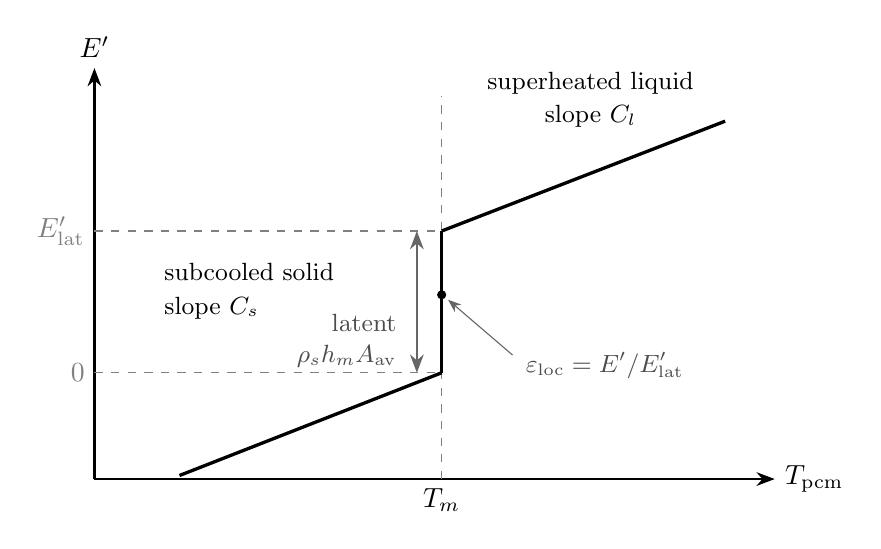
\begin{tikzpicture}[>=Stealth, scale=0.9]
  \draw[->,thick] (0,0) -- (9.6,0) node[right] {$\Tpcm$};
  \draw[->,thick] (0,0) -- (0,5.8) node[above] {$E'$};
  \draw[dashed,gray] (4.9,0) -- (4.9,5.4);
  \node[below] at (4.9,0) {$T_{m}$};
  \draw[dashed,gray] (0,1.5) -- (4.9,1.5) node[pos=0,left] {$0$};
  \draw[dashed,gray] (0,3.5) -- (4.9,3.5) node[pos=0,left] {$\Elat$};
  \draw[very thick] (1.2,0.05) -- (4.9,1.5);
  \draw[very thick] (4.9,1.5) -- (4.9,3.5);
  \draw[very thick] (4.9,3.5) -- (8.9,5.05);
  \node[align=left,font=\small,anchor=west] at (0.85,2.65)
    {subcooled solid\\[1pt] slope $C_{s}$};
  \node[align=center,font=\small] at (7.0,5.35)
    {superheated liquid\\[1pt] slope $C_{l}$};
  \draw[<->,thick,black!60] (4.55,1.5) -- (4.55,3.5);
  \node[font=\small,align=right,anchor=east,black!70] at (4.4,1.95)
    {latent\\$\rho_s\hm\Aav$};
  \filldraw (4.9,2.6) circle (1.6pt);
  \draw[->,black!60] (5.9,1.75) -- (4.99,2.53);
  \node[font=\small,align=left,anchor=west,black!70] at (5.95,1.6)
    {$\eloc=E'/\Elat$};
\end{tikzpicture}
\caption{Constitutive relation of the segment state, Eq.~\eqref{eq:enth-curve}.
Read as $T(E')$ it is single-valued; position along the vertical segment is
the melted fraction.}
\label{fig:enthalpy-curve}
\end{figure}

\subsubsection{Segment energy balances and closure}
\label{sec:segment}

The developed length is divided into $n_s$ segments of length
$\Delta s=\Ltube/n_s$. For segment $j$, spanning $[s_j,s_{j+1}]$, two control
volumes share the tube wall (Fig.~\ref{fig:cv}): CV1, the PCM belonging to the
segment, which is closed and stationary; and CV2, the water within the tube
over the same interval, which enters at $T_j$ and leaves at $T_{j+1}$. Let
$q'_j$ denote the heat rate per unit length crossing from CV2 into CV1.

\begin{figure}[htbp]
\centering
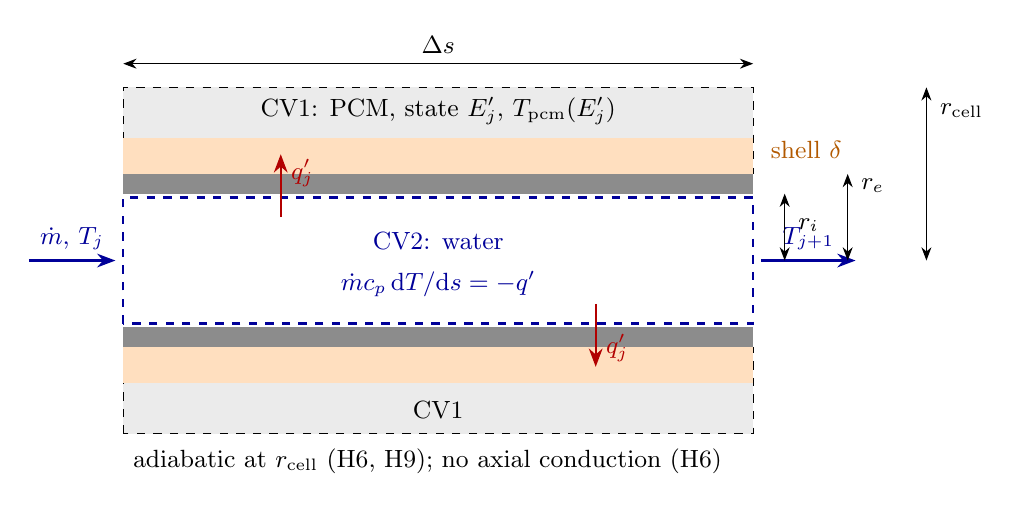
\begin{tikzpicture}[>=Stealth, font=\small, scale=1.0]
  % PCM annulus (CV1)
  \fill[black!8] (0,1.1) rectangle (8,2.2);
  \fill[black!8] (0,-2.2) rectangle (8,-1.1);
  \draw[dashed] (0,1.1) rectangle (8,2.2);
  \draw[dashed] (0,-2.2) rectangle (8,-1.1);
  % melt shell
  \fill[orange!25] (0,1.1) rectangle (8,1.55);
  \fill[orange!25] (0,-1.55) rectangle (8,-1.1);
  % tube wall
  \fill[black!45] (0,0.85) rectangle (8,1.1);
  \fill[black!45] (0,-1.1) rectangle (8,-0.85);
  % water (CV2)
  \draw[thick,blue!60!black,dashed] (0,-0.8) rectangle (8,0.8);
  \draw[->,thick,blue!60!black] (-1.2,0) -- (-0.1,0) node[midway,above] {$\md,\,T_j$};
  \draw[->,thick,blue!60!black] (8.1,0) -- (9.3,0) node[midway,above] {$T_{j+1}$};
  \node[blue!60!black] at (4,0.25) {CV2: water};
  \node[blue!60!black] at (4,-0.3) {$\md c_p\,\mathrm{d}T/\mathrm{d}s=-q'$};
  \node at (4,1.9) {CV1: PCM, state $E'_j$, $\Tpcm(E'_j)$};
  \node at (4,-1.9) {CV1};
  \draw[->,thick,red!70!black] (2,0.55) -- (2,1.35) node[right,pos=0.7] {$q'_j$};
  \draw[->,thick,red!70!black] (6,-0.55) -- (6,-1.35) node[right,pos=0.7] {$q'_j$};
  % dimensions
  \draw[<->] (0,2.5) -- (8,2.5) node[midway,above] {$\Delta s$};
  \draw[<->] (8.4,0) -- (8.4,0.85);  \node[right] at (8.45,0.45) {$r_i$};
  \draw[<->] (9.2,0) -- (9.2,1.1);   \node[right] at (9.25,0.95) {$r_e$};
  \node[right,orange!70!black] at (8.1,1.4) {shell $\delta$};
  \draw[<->] (10.2,0) -- (10.2,2.2); \node[right] at (10.25,1.9) {$r_\mathrm{cell}$};
  \node[anchor=west] at (0,-2.55) {adiabatic at $r_\mathrm{cell}$ (H6, H9); no axial conduction (H6)};
\end{tikzpicture}
\caption{Control volumes of segment $j$ (axial section of one leg; fins not
shown). CV1 is the PCM belonging to the segment, CV2 the water over the same
interval. The shaded shell adjacent to the tube is the conduction path of
Eq.~\eqref{eq:shell-choice}.}
\label{fig:cv}
\end{figure}

\paragraph{PCM balance} CV1 does no work and, by H6, exchanges heat only
through the tube wall, so the first law reduces to
\begin{equation}
  \frac{\mathrm{d}E'_j}{\mathrm{d}t}=q'_j .
  \label{eq:pcm-balance}
\end{equation}

\paragraph{Water balance} For incompressible single-phase flow without
viscous dissipation, the energy equation per unit tube length is
\begin{equation}
  \rho_\mathrm{w}A_\mathrm{flow}c_{p}\frac{\partial T}{\partial t}
  +\md c_{p}\frac{\partial T}{\partial s}=-q'(s),
  \label{eq:fluid-pde}
\end{equation}
with $A_\mathrm{flow}=\pi r_i^{2}$. Hypothesis H7 drops the storage term. The
approximation rests on the separation between the transit time of the water
through the hairpin, $\Ltube\rho_\mathrm{w}A_\mathrm{flow}/\md$, and the time
over which the PCM state evolves, $t_\mathrm{ch}$ or $t_\mathrm{dc}$, and on
the ratio of the energy held in the water to the latent inventory,
$\rho_\mathrm{w}A_\mathrm{flow}c_{p}\Delta T/\Elat$; both are quantified for
the reference case in Section~\ref{sec:conditions}. Its cost is that the
start-up transient of about one transit time at the beginning of each
half-cycle is not resolved.

The local heat flux is closed on the resistance network of
Section~\ref{sec:network}, referred to the inner tube area,
\begin{equation}
  q'(s)=2\pi r_i\,\Ui\left[T(s)-\Tpcm\right],
  \label{eq:local-flux}
\end{equation}
where CV1 presents the single temperature $\Tpcm(E'_j)$ over the whole
segment (H1). The perimeter is the inner perimeter $2\pi r_i$ because $\Ui$ is
referred to the inner area and already contains the finned outer surface.

\paragraph{Integration across the segment} With $\Tpcm$ and $\Ui$ held
constant over the segment, the steady form of Eq.~\eqref{eq:fluid-pde} with
Eq.~\eqref{eq:local-flux} is a linear ordinary differential equation in $s$
whose solution is the single-stream exchanger result
\begin{equation}
  T_{j+1}=\Tpcm+\left(T_j-\Tpcm\right)e^{-\NTU_j},
  \qquad
  \NTU_j=\frac{2\pi r_i\,\Ui\,\Delta s}{\md c_{p}} .
  \label{eq:ntu}
\end{equation}
The water is a stream of finite capacity rate $\md c_p$ exchanging heat with
an isothermal reservoir; the effectiveness is $1-e^{-\NTU}$.

\paragraph{Closure} The heat given up by the water over the segment is the
enthalpy it loses, $\md c_p(T_j-T_{j+1})=q'_j\Delta s$, so that
\begin{equation}
  q'_j=K_j\left(T_j-\Tpcm\right),
  \qquad
  K_j=\frac{\md c_{p}\left(1-e^{-\NTU_j}\right)}{\Delta s},
  \label{eq:K}
\end{equation}
and substituting into Eq.~\eqref{eq:pcm-balance} gives the segment equation
\begin{equation}
  \frac{\mathrm{d}E'_j}{\mathrm{d}t}=K_j\left[T_j-\Tpcm(E'_j)\right],
  \label{eq:ode}
\end{equation}
with one unknown per segment; $T_j$ is handed down by the upstream segment and
$K_j$ depends on the state through $\Ui$. The water temperature is then
advanced by
\begin{equation}
  T_{j+1}=T_j-\frac{q'_j\,\Delta s}{\md c_{p}} .
  \label{eq:T-march}
\end{equation}

The closure of Eq.~\eqref{eq:K} is not the product
$2\pi r_i\Ui$ that results from evaluating Eq.~\eqref{eq:local-flux} at the
segment inlet. The ratio of the two is
\begin{equation}
  \frac{K_j}{2\pi r_i\Ui}=\frac{1-e^{-\NTU_j}}{\NTU_j}\le 1 .
  \label{eq:K-ratio}
\end{equation}
As $\NTU\to0$ the ratio tends to unity; as $\NTU\to\infty$, $K\to\md
c_p/\Delta s$, a limit set by the capacity rate of the water rather than by the
wall. The product form has no such limit and permits $T_{j+1}<\Tpcm$, i.e.\
heat transfer from cold to hot, at a rate that increases without bound as the
wall conductance improves. The discrepancy is largest where the phase-change
shell is thin and the exchanger most effective.

\subsubsection{Thermal resistance network}
\label{sec:network}

The overall heat transfer coefficient referred to the inner tube area is the
series combination of internal convection, internal fouling, wall conduction
and the PCM-side resistance of the finned outer surface,
\begin{equation}
  \frac{1}{\Ui}=\frac{1}{h_i}+R''_{f,i}+\frac{r_i}{k_\mathrm{wall}}\ln\frac{r_e}{r_i}
  +\frac{2\pi r_i}{P_T\,\etao\,h_e},
  \qquad
  h_e=\frac{k}{r_e\ln\left(1+\delta/r_e\right)},
  \label{eq:Ui}
\end{equation}
where $h_e$ is the conductance of a cylindrical PCM shell of thickness $\delta$
and conductivity $k$, referred to the outer tube surface, and the factor
$2\pi r_i/(P_T\etao)$ transfers it to the inner area.

\paragraph{Internal convection} The coefficient $h_i$ is evaluated locally at
the bulk water temperature $T_j$ of each segment and at each time level. For
$\mathrm{Re}=4\md/(\pi D_i\mu)\ge2300$ the Gnielinski correlation
\cite{Gnielinski1976} is used with the Petukhov friction factor,
\begin{equation}
  \mathrm{Nu}=\frac{(f/8)(\mathrm{Re}-1000)\mathrm{Pr}}
    {1+12.7\sqrt{f/8}\left(\mathrm{Pr}^{2/3}-1\right)},
  \qquad
  f=\left(0.79\ln\mathrm{Re}-1.64\right)^{-2},
  \label{eq:gnielinski}
\end{equation}
and $\mathrm{Nu}=3.66$ otherwise, with $h_i=\mathrm{Nu}\,k_\mathrm{w}/D_i$, where $k_\mathrm{w}$ is the conductivity of water. Properties are evaluated at $T_j$ and $p_\mathrm{w}$.

\paragraph{Fins} With $n_f$ longitudinal fins per leg, the finned perimeter,
the fin efficiency and the overall surface efficiency are
\begin{gather}
  P_T=2\pi r_e+2n_fL_f,
  \qquad
  \etao=1-\frac{n_fA_f}{A_t}\left(1-\etaf\right),
  \label{eq:fins}\\
  \etaf=\frac{\tanh(mL_c)}{mL_c},
  \qquad m=\sqrt{\frac{2h_e}{k_\mathrm{fin}t_f}},
  \qquad L_c=L_f+\frac{t_f}{2},
  \label{eq:fin-eff}
\end{gather}
with $A_f=(2L_f+t_f)\Delta s$ the surface of one fin and $A_t=P_T\Delta s$
the total outer surface of the segment \cite{Incropera}. The fin conductivity
is taken equal to that of the tube wall, $k_\mathrm{fin}=k_\mathrm{wall}$.

\paragraph{Shell thickness from the melted area}
The fin metal occupies part of the annulus about the tube, so the melted area
and the shell thickness are related by
\begin{equation}
  A=\pi\left[(r_e+\delta)^{2}-r_e^{2}\right]-n_ft_f\min(\delta,L_f),
  \label{eq:area-fins}
\end{equation}
which is inverted in closed form on each branch:
\begin{align}
  \delta\le L_f:&\quad
    \pi\delta^{2}+\left(2\pi r_e-n_ft_f\right)\delta-A=0,
  \label{eq:delta-in}\\
  \delta>L_f:&\quad
    \pi\delta^{2}+2\pi r_e\delta-\left(A+n_ft_fL_f\right)=0 .
  \label{eq:delta-out}
\end{align}

\paragraph{Conduction path: which shell the heat crosses}
The PCM-side term in Eq.~\eqref{eq:Ui} is the resistance of a shell growing
outward from the tube wall, so the model must specify the material of which
that shell consists. Because the tube is the driven boundary in both
half-cycles, the phase-change front always originates at the wall and moves
outward. During melting the shell is liquid and its area is the melted area;
during freezing the shell is the newly frozen solid and its area is the solid
area, the remaining liquid being displaced beyond the front and out of the
conduction path. For a segment in the two-phase branch,
\begin{equation}
  \left(A,\,k\right)=
  \begin{cases}
    \left(\Amelt,\;k_{l}\right), & T_j>\Tpcm\quad\text{(melting)},\\[3pt]
    \left(\Aav-\Amelt,\;k_{s}\right), & T_j<\Tpcm\quad\text{(freezing)},
  \end{cases}
  \label{eq:shell-choice}
\end{equation}
and $\delta$ follows from Eqs.~\eqref{eq:delta-in}--\eqref{eq:delta-out}. The
direction is taken from the sign of the driving temperature difference, which
is known before the conductance is formed. Equation~\eqref{eq:shell-choice}
gives the correct limits without special treatment: a fully solid segment
beginning to melt and a fully liquid segment beginning to freeze both have
$\delta=0$. Using the melted area in both directions, as in a formulation
written for melting and not revisited, reverses the freezing half-cycle in
time: a segment frozen solid is assigned zero resistance where the physical
resistance is greatest.

\paragraph{Single-phase segments: a mean-to-surface resistance}
A segment in either sensible branch contains no front, and
Eq.~\eqref{eq:shell-choice} does not apply. In that case $\Tpcm$ is the
volume-mean temperature of the cell, because the state is the cell's total
enthalpy, and the resistance consistent with a mean temperature is the
mean-to-surface resistance. Consider the cell as an annulus
$r_e\le r\le r_\mathrm{cell}$, adiabatic at $r_\mathrm{cell}$ (a symmetry
surface with the neighbouring cell), storing sensible heat at a uniform
volumetric rate $\dot s$. Under quasi-steady conditions (H2) the heat crossing
radius $r$ is that stored beyond it,
$-k\,2\pi r\,\mathrm{d}T/\mathrm{d}r=\dot s\pi(r_\mathrm{cell}^{2}-r^{2})$,
which integrates to
\begin{equation}
  T(r_e)-T(r)=\frac{\dot s}{2k}
  \left[r_\mathrm{cell}^{2}\ln\frac{r}{r_e}-\frac{r^{2}-r_e^{2}}{2}\right].
  \label{eq:bulk-profile}
\end{equation}
Averaging over the cell volume and dividing by
$Q'=\dot s\pi(r_\mathrm{cell}^{2}-r_e^{2})$ gives
$R'_\mathrm{bulk}=S/(2\pi k)$, with the geometric shape factor
\begin{equation}
  S=\frac{4\beta^{4}\ln\beta-3\beta^{4}+4\beta^{2}-1}
         {4\left(\beta^{2}-1\right)^{2}},
  \qquad \beta=\frac{r_\mathrm{cell}}{r_e}.
  \label{eq:shape-factor}
\end{equation}
The conductivity cancels, so the same $S$ serves both phases. For a thin
annulus of thickness $L=r_\mathrm{cell}-r_e\ll r_e$, $S\to L/(3r_e)$ and
$R'_\mathrm{bulk}\to L/(3kA)$ with $A=2\pi r_e$ per unit length, which is the
mean-to-surface resistance of a plane slab with uniform generation. The
resistance enters Eq.~\eqref{eq:Ui} as an equivalent thickness
$\delta_\mathrm{eq}=r_e\left(e^{S}-1\right)$, with $k=k_s$ for subcooled
solid and $k=k_l$ for superheated liquid, so that the fin relations apply
unchanged.

The PCM-side resistance is consequently discontinuous at the branch
boundaries. As $\eloc\to1^{-}$ during melting the front approaches
$r_\mathrm{cell}$ and $R'\to\ln\beta/(2\pi k_l)$, whereas once the segment is
superheated $R'=S/(2\pi k_l)$. The discontinuity reflects the change in the
reference temperature, from the front to the volume mean, rather than a
physical event, and the heat flux remains bounded because $K$ is limited by the
capacity rate, Eq.~\eqref{eq:K}.

\paragraph{Limitation of a single front} After the first half-cycle from a
uniformly solid store, the phase distribution within a cell is in general
three-region: at cyclic steady state a charge begins with residual liquid in
the outer part of the cell, so that melting produces liquid at the tube, solid
in the middle and liquid beyond it. Equation~\eqref{eq:shell-choice} is the
better of the two single-front approximations, not a resolution of this
geometry; this is the content of H5.

%-----------------------------------------------------------------------
\subsection{Charging period}
\label{sec:BB_ch}
%-----------------------------------------------------------------------

During charging the water enters every hairpin at $s=0$ with temperature
$T_\mathrm{4c}$, Eq.~\eqref{eq:inlets}, and mass flow rate $\md_\mathrm{ch}$,
Eq.~\eqref{eq:mdot}, and the segment equations
\eqref{eq:ode}--\eqref{eq:T-march} are marched in the direction of increasing
$s$ against the cascade of Eq.~\eqref{eq:cascade}. Segments in which
$T_j>\Tpcm$ melt through a liquid shell of conductivity $k_l$; segments that
have completed melting superheat, their driving difference $T_j-\Tpcm$
decreases, and the heat they no longer absorb is carried downstream. The
energy absorbed by the field over the charging period and the melted fraction
of the store at its end are
\begin{gather}
  \Delta E_\mathrm{ch}=\Nw\,n_t\int_{0}^{t_\mathrm{ch}}\sum_{j=1}^{n_s}
     q'_j(t)\,\Delta s\,\mathrm{d}t
   =\Nw\,n_t\,\Delta s\sum_{j=1}^{n_s}\left[E'_j(t_\mathrm{ch})-E'_j(0)\right],
  \label{eq:Ech}\\
  \bar\varepsilon_\mathrm{ch}=\frac1{n_s}\sum_{j=1}^{n_s}
     \varepsilon_{\mathrm{loc},j}(t_\mathrm{ch}),
  \label{eq:eps-ch}
\end{gather}
where the second equality holds exactly under the integrator of
Section~\ref{sec:integration}. The water leaves the field at the
time-dependent temperature $T_{n_s+1}(t)$; its flow-averaged value,
\begin{equation}
  \overline{T}_\mathrm{2c}=\frac{1}{t_\mathrm{ch}}\int_{0}^{t_\mathrm{ch}}
     T_{n_s+1}(t)\,\mathrm{d}t,
  \label{eq:Tout-mean}
\end{equation}
is the temperature at which the water returns to the HTHP condenser and is
reported alongside the nominal value $T_\mathrm{2c}$ of
Table~\ref{tab:closure}. At constant $\md$ and $c_p$ the flow average reduces
to the time average; on a logarithmic time grid it must be weighted by the
step length.

%-----------------------------------------------------------------------
\subsection{Discharging period}
\label{sec:BB_dc}
%-----------------------------------------------------------------------

During discharging the flow reverses. The water enters at $s=\Ltube$ with
temperature $T_\mathrm{3d}$, Eq.~\eqref{eq:inlets}, and mass flow rate
$\md_\mathrm{dc}$, and meets the layer of lowest melting temperature first.
The governing equations are those of the charging period, with two
differences. First, in segments where $T_j<\Tpcm$ the conduction path is the
frozen shell with conductivity $k_s$, Eq.~\eqref{eq:shell-choice}. Second, the
march proceeds in the direction of decreasing $s$, so both the melting
temperatures and the initial state, which is the state at the end of the
preceding charge, are mirrored with the march index; since $E'$ is measured
from a datum at each segment's own $T_m$, mirroring the cascade without
mirroring the state would displace the datum by up to the full cascade span.
The energy released by the field and the residual melted fraction are
\begin{equation}
  \Delta E_\mathrm{dc}=-\Nw\,n_t\,\Delta s\sum_{j=1}^{n_s}
     \left[E'_j(t_\mathrm{dc})-E'_j(0)\right],
  \qquad
  \bar\varepsilon_\mathrm{dc}=\frac1{n_s}\sum_{j=1}^{n_s}
     \varepsilon_{\mathrm{loc},j}(t_\mathrm{dc}),
  \label{eq:Edc}
\end{equation}
and the flow-averaged outlet $\overline{T}_\mathrm{2d}$, defined as in
Eq.~\eqref{eq:Tout-mean}, is the temperature at which the water reaches the ORC
evaporator.

Idle periods between the half-cycles, if any, leave the state unchanged under
H6, since the store is adiabatic and carries no axial conduction.

%-----------------------------------------------------------------------
\subsection{Pressure drop and pumping power}
\label{sec:pumping}
%-----------------------------------------------------------------------

The pressure drop over one hairpin is the sum of distributed friction over the
developed length and local losses at the entrance, the return bends and the
exit,
\begin{equation}
  \Delta p_f=\left(f\,\frac{\Ltube}{D_i}+\sum K_\mathrm{loc}\right)
            \frac{\rho_\mathrm{w}\bar u^{2}}{2},
  \qquad
  \bar u=\frac{\md}{\rho_\mathrm{w}\pi r_i^{2}},
  \label{eq:dp}
\end{equation}
with $\sum K_\mathrm{loc}=0.5+2(2.2)+1.0$ \chk{one 180$^\circ$ return per
hairpin, or two?} and the Darcy friction factor of a smooth tube:
$f=64/\mathrm{Re}$ for $\mathrm{Re}<2000$; $f=0.3164\,\mathrm{Re}^{-1/4}$
(Blasius) for $\mathrm{Re}\le10^{5}$; and
$f=0.0032+0.221\,\mathrm{Re}^{-0.237}$ for $10^{5}<\mathrm{Re}\le10^{6}$.
\chk{Ref.~\cite{KoIHTC2026} states Haaland \cite{Haaland1983}; the code uses the
smooth-tube forms above. Choose one and make paper and code agree.} Water
properties are evaluated at the loop pressure and the mean of the inlet and
the flow-averaged outlet temperatures. The hydraulic pumping power of the
field in each half-cycle is
\begin{equation}
  \dot W_{f}=\Nw\,n_t\,\frac{\md}{\rho_\mathrm{w}}\,\Delta p_f ,
  \label{eq:Wf}
\end{equation}
\chk{no pump efficiency is applied; add $\eta_\mathrm{pump}$ or state it.}
evaluated with $\md_\mathrm{ch}$ and $\md_\mathrm{dc}$ respectively and
entering Eqs.~\eqref{eq:etaT}--\eqref{eq:rte}. Hydrostatic contributions
cancel over a closed hairpin.


%-----------------------------------------------------------------------
\subsection{Exergy analysis}
\label{sec:exergy}
%-----------------------------------------------------------------------

At cyclic steady state the store returns every unit of energy it absorbs,
Eq.~\eqref{eq:css-unity}, so the first law cannot express what the store, or
any other component, costs. The cost of each component is the exergy it
destroys, and the analysis below allocates the exergy input of the plant over
one complete cycle to the net electrical output, to a discarded stream and to
the destruction in each component.

\subsubsection{Dead state and reservoirs}

The dead state is taken as the ORC heat sink, $T_0=T_\mathrm{sink}$, at the
pressure of each stream. It is the lowest temperature in the system, so all
stream exergies are non-negative, and the heat rejected in the ORC condenser
carries no exergy. The plant exchanges heat with two reservoirs: the sink, at
the dead state, and the geothermal stream that supplies the HTHP evaporator.
The latter is not at the dead state and is an exergy input to the plant. The
exergy given up by a stream of water cooling from $T_a$ to $T_b$ at
$p_\mathrm{w}$ is
\begin{equation}
  \Exd_\mathrm{w}(T_a,T_b)=\md\left[h_\mathrm{w}(T_a)-h_\mathrm{w}(T_b)
     -T_0\left(s_\mathrm{w}(T_a)-s_\mathrm{w}(T_b)\right)\right],
  \label{eq:ex-stream}
\end{equation}
and $\Exd_\mathrm{w}(T_a,T_0)$ is the exergy of the stream relative to the
dead state.

\subsubsection{The geothermal source as a finite resource}
\label{sec:geo}

The heat-pump source is co-produced or geothermal water drawn from producing
wells at $T_\mathrm{source}$ and reinjected at
$T_\mathrm{4a}=T_\mathrm{source}-\Delta T_\mathrm{3A,4A}$. Its flow rate is not
prescribed but derived from the evaporator duty, in the same way as $\Nw$ is
derived from the storage duty. With
$\md_\mathrm{ref}=\dot Q_\mathrm{out,HP}/(h_\mathrm{2h}-h_\mathrm{3h})$ the
refrigerant flow through the condenser,
\begin{gather}
  \dot Q_\mathrm{src}=\md_\mathrm{ref}\left(1-x_\mathrm{8h}\right)
     \left(h_\mathrm{13h}-h_\mathrm{4h}\right),
  \notag\\
  \md_\mathrm{geo}=\frac{\dot Q_\mathrm{src}}
     {h_\mathrm{w}(T_\mathrm{source})-h_\mathrm{w}(T_\mathrm{4a})},
  \qquad
  N_\mathrm{geo}=\frac{\md_\mathrm{geo}}{\md_\mathrm{geo,well}},
  \label{eq:mgeo}
\end{gather}
where $\md_\mathrm{geo,well}$ is the yield of one producing well. Deriving
$\md_\mathrm{geo}$ places the uncertainty in the per-well yield, which is a
field-measured quantity, rather than in a plant-level flow rate; since the
source exergy is homogeneous of degree one in $\md_\mathrm{geo}$, the choice
does not affect the exergetic efficiencies below. $\Delta T_\mathrm{3A,4A}$ is
bounded above by a minimum reinjection temperature
$T_\mathrm{reinj,min}$, which represents formation constraints such as scaling
and injectivity.

Two conventions are possible for the exergy charged to the plant for the
geothermal stream. Under the \emph{resource} convention adopted here, the plant
is charged with the full exergy of the produced stream relative to the dead
state, and the exergy still carried by the reinjected stream is booked as a
loss attributed to no component:
\begin{gather}
  \Exd_\mathrm{geo}=\Exd_\mathrm{w}\!\left(T_\mathrm{source},T_0\right),
  \qquad
  \Exd_\mathrm{reinj}=\Exd_\mathrm{w}\!\left(T_\mathrm{4a},T_0\right),
  \notag\\
  u_\mathrm{geo}=1-\frac{\Exd_\mathrm{reinj}}{\Exd_\mathrm{geo}},
  \label{eq:ex-geo}
\end{gather}
where both terms are evaluated with $\md_\mathrm{geo}$ and $u_\mathrm{geo}$ is
the fraction of the resource that the plant uses. Under the alternative
\emph{stripped} convention, only the exergy removed in the evaporator,
$\Exd_\mathrm{geo}-\Exd_\mathrm{reinj}=\Exd_\mathrm{w}(T_\mathrm{source},
T_\mathrm{4a})$, is charged and reinjection is free. The resource convention is
appropriate for a dedicated producer, which is drilled, completed and operated
whether or not the exergy it lifts is used. The distinction is not cosmetic:
the two conventions give opposite guidance on $\Delta T_\mathrm{3A,4A}$
(Section~\ref{sec:res-exergy}). Under the stripped convention the exergetic
efficiency decreases monotonically with $\Delta T_\mathrm{3A,4A}$, which drives
the design toward the smallest cooling of the source and hence the largest
geothermal flow and well count; under the resource convention it has an
interior maximum.

\subsubsection{Exergy balance over a cycle}

Over one cycle at CSS the exergy of the store returns to its initial value, and
the balance for the whole plant reads
\begin{equation}
  W_\mathrm{el,in}+\Ex_\mathrm{geo}
  =W_\mathrm{el,out}+\Ex_\mathrm{reinj}+\sum_{j}I_{j},
  \label{eq:ex-balance}
\end{equation}
with $W_\mathrm{el,in}=\dot W_\mathrm{el,in}t_\mathrm{ch}$,
$W_\mathrm{el,out}=\dot W_\mathrm{el,out}t_\mathrm{dc}$,
$\Ex_\mathrm{geo}=\Exd_\mathrm{geo}t_\mathrm{ch}$ and
$\Ex_\mathrm{reinj}=\Exd_\mathrm{reinj}t_\mathrm{ch}$, all evaluated on the
energy the field actually moves at cyclic steady state rather than on the
target duties. The
destruction in component $j$ follows from the Gouy--Stodola theorem,
$I_j=T_0\,S_{\mathrm{gen},j}$, with the entropy generation computed from the
state points and flow fractions of that component alone.

\paragraph{Heat pump} Per unit mass through the condenser, and with the water
flow rates referred to $\md_\mathrm{ref}$,
\begin{align}
  s_{\mathrm{gen,C,HP}}&=s_\mathrm{2h}-s_\mathrm{6h},\notag\\
  s_{\mathrm{gen,C,LP}}&=\left(1-x_\mathrm{8h}\right)\left(s_\mathrm{5h}-s_\mathrm{1h}\right),
  \notag\\
  s_{\mathrm{gen,V,7-8}}&=s_\mathrm{8h}-s_\mathrm{7h},\notag\\
  s_{\mathrm{gen,V,9-4}}&=\left(1-x_\mathrm{8h}\right)\left(s_\mathrm{4h}-s_\mathrm{9h}\right),
  \notag\\
  s_{\mathrm{gen,sep}}&=x_\mathrm{8h}s_\mathrm{10h}+\left(1-x_\mathrm{8h}\right)s_\mathrm{9h}-s_\mathrm{8h},\notag\\
  s_{\mathrm{gen,R1}}&=\left(s_\mathrm{12h}-s_\mathrm{3h}\right)+x_\mathrm{8h}\left(s_\mathrm{11h}-s_\mathrm{10h}\right),
  \notag\\
  s_{\mathrm{gen,R2}}&=\left(s_\mathrm{7h}-s_\mathrm{12h}\right)+\left(1-x_\mathrm{8h}\right)\left(s_\mathrm{1h}-s_\mathrm{13h}\right),\notag\\
  s_{\mathrm{gen,cond}}&=\left(s_\mathrm{3h}-s_\mathrm{2h}\right)
     +\frac{\md_\mathrm{w,ch}^\mathrm{tot}}{\md_\mathrm{ref}}
      \left[s_\mathrm{w}(T_\mathrm{3c})-s_\mathrm{w}(T_\mathrm{2c})\right],
  \notag\\
  s_{\mathrm{gen,evap}}&=\left(1-x_\mathrm{8h}\right)\left(s_\mathrm{13h}-s_\mathrm{4h}\right)
     +\frac{\md_\mathrm{geo}}{\md_\mathrm{ref}}
      \left[s_\mathrm{w}(T_\mathrm{4a})-s_\mathrm{w}(T_\mathrm{source})\right],
  \label{eq:sgen-hp}
\end{align}
where $\md_\mathrm{w,ch}^\mathrm{tot}=\Nw n_t\md_\mathrm{ch}$ is the total
water flow, and $I_j=T_0\md_\mathrm{ref}s_{\mathrm{gen},j}t_\mathrm{ch}$. The
motor loss is
$I_\mathrm{mot}=(\dot W_\mathrm{el,in}-\dot W_\mathrm{C})t_\mathrm{ch}$, with
$\dot W_\mathrm{C}=\md_\mathrm{ref}[(h_\mathrm{2h}-h_\mathrm{6h})
+(1-x_\mathrm{8h})(h_\mathrm{5h}-h_\mathrm{1h})]$ the shaft power of the two
compressors.

\paragraph{Organic Rankine cycle} Per unit mass through the high-pressure
turbine, whose flow rate is
$\md_\mathrm{orc}=\dot Q_\mathrm{in,ORC}/[(h_\mathrm{3e}-h_\mathrm{10e})
+y(h_\mathrm{6e}-h_\mathrm{5e})]$,
\begin{align}
  s_{\mathrm{gen,T1}}&=s_\mathrm{5e}-s_\mathrm{3e},\notag\\
  s_{\mathrm{gen,T2}}&=y\left(s_\mathrm{4e}-s_\mathrm{6e}\right),
  \notag\\
  s_{\mathrm{gen,P1}}&=y\left(s_\mathrm{2e}-s_\mathrm{1e}\right),\notag\\
  s_{\mathrm{gen,P2}}&=\left(1-y\right)\left(s_\mathrm{8e}-s_\mathrm{7e}\right),
  \notag\\
  s_{\mathrm{gen,FH}}&=\left(1-y\right)\left(s_\mathrm{7e}-s_\mathrm{5e}\right)
     +y\left(s_\mathrm{9e}-s_\mathrm{2e}\right),\notag\\
  s_{\mathrm{gen,mix}}&=s_\mathrm{10e}-y\,s_\mathrm{9e}-\left(1-y\right)s_\mathrm{8e},
  \notag\\
  s_{\mathrm{gen,evap}}&=\left(s_\mathrm{3e}-s_\mathrm{10e}\right)
     +y\left(s_\mathrm{6e}-s_\mathrm{5e}\right)
     +\frac{\md_\mathrm{w,dc}^\mathrm{tot}}{\md_\mathrm{orc}}
      \left[s_\mathrm{w}(T_\mathrm{3d})-s_\mathrm{w}(T_\mathrm{2d})\right],\notag\\
  s_{\mathrm{gen,cond}}&=y\left(s_\mathrm{1e}-s_\mathrm{4e}\right)
     +\frac{y\left(h_\mathrm{4e}-h_\mathrm{1e}\right)}{T_0},
  \label{eq:sgen-orc}
\end{align}
with $I_j=T_0\md_\mathrm{orc}s_{\mathrm{gen},j}t_\mathrm{dc}$. Because the sink
is at the dead state, the whole exergy of the heat rejected in the condenser is
destroyed there. The generator loss is
$I_\mathrm{gen}=(\dot W_\mathrm{T}-\dot W_\mathrm{el,out})t_\mathrm{dc}$, with
$\dot W_\mathrm{T}$ the net shaft power of the turbines less the pumps.

\paragraph{Borehole field} The destruction in the borehole field is obtained as
the difference between the exergy the water gives up during charging and the
exergy it recovers during discharging,
\begin{equation}
  I_\mathrm{BB}=\Exd_\mathrm{w}^\mathrm{tot}\!\left(T_\mathrm{3c},T_\mathrm{2c}\right)t_\mathrm{ch}
   -\Exd_\mathrm{w}^\mathrm{tot}\!\left(T_\mathrm{2d},T_\mathrm{3d}\right)t_\mathrm{dc},
  \label{eq:I-BB}
\end{equation}
evaluated with the total water flow of each half-cycle. The expression is exact
at CSS, because the exergy of the PCM returns to its initial value over the
cycle and no entropy function of the PCM is required. It aggregates the
destruction over the depth and duration of the cycle and does not locate it;
resolving it in $s$ and $t$ requires an entropy relation $s(E')$ consistent
with Eq.~\eqref{eq:enth-curve}. \todo{independent evaluation of $I_\mathrm{BB}$
from $s(E')$ integrated over the march.}

\subsubsection{Exergetic efficiencies}

The round-trip efficiency, Eq.~\eqref{eq:rte}, books the geothermal source as
free. The exergetic efficiency under the resource convention charges it, and
the stripped value is reported alongside for comparison:
\begin{equation}
  \psi=\frac{W_\mathrm{el,out}-W_\mathrm{f,dc}}
            {W_\mathrm{el,in}+W_\mathrm{f,ch}+\Ex_\mathrm{geo}},
  \qquad
  \psi_\mathrm{str}=\frac{W_\mathrm{el,out}-W_\mathrm{f,dc}}
            {W_\mathrm{el,in}+W_\mathrm{f,ch}+\Ex_\mathrm{geo}-\Ex_\mathrm{reinj}},
  \label{eq:psi}
\end{equation}
where $W_\mathrm{f}=\dot W_\mathrm{f}t$ are the pumping energies of the
borehole field, so that $\psi$ and RTE share the same boundary and differ only
in the charge for the geothermal stream. The geothermal well count
$N_\mathrm{geo}$, Eq.~\eqref{eq:mgeo}, is reported together with $\Nw$, and the
total number of wells per unit of net output,
$(\Nw+N_\mathrm{geo})/\dot W_\mathrm{el,out}$, is carried as a design indicator:
a comparison based on RTE alone favours designs that buy COP with an
arbitrarily large geothermal flow.

Including the pumping terms is what makes $\psi$ and RTE share a control
volume, and it is not a small correction: in the reference case $\psi$ is
\num{0.246} if they are omitted and \num{0.236} if they are charged. The code
was brought onto this definition at v0.15, and a build-time check now asserts
that the RTE computed inside the audit and the RTE computed from the marched
field agree to the last bit --- a cross-check that exists because this
discrepancy was found while writing the present section rather than by any
test in the code.

%=======================================================================
\section{Mathematical implementation}
\label{sec:implementation}
%=======================================================================

\subsection{Time integration}
\label{sec:integration}

The segment equation~\eqref{eq:ode} is nonlinear, because $\Tpcm(E')$ is
piecewise, but it is affine within each branch of
Eq.~\eqref{eq:enth-curve}. Over a time step $\Delta t$ the upstream water
temperature $T_j$ and the conductance $K_j$ are held at their values at the
beginning of the step, which are obtained by marching
Eqs.~\eqref{eq:Ui}, \eqref{eq:ntu}, \eqref{eq:K} and \eqref{eq:T-march} from
the inlet with the state frozen. The distinction between the branches governs
the choice of integrator.

\paragraph{Explicit stepping} On the latent plateau $\Tpcm=T_m$ does not depend
on $E'$, the segment behaves as though its heat capacity were infinite, and
Eq.~\eqref{eq:ode} reduces to $\mathrm{d}E'/\mathrm{d}t=K(T_j-T_m)$, for which
an explicit Euler step is exact. A model whose state is the melted area
occupies this regime permanently, which is why explicit stepping is adequate
for such models. On the sensible branches Eq.~\eqref{eq:ode} is a linear
relaxation with time constant $\tau=C/K$, and explicit Euler is stable only
for $\Delta t<2\tau$ and monotone only for $\Delta t<\tau$. The time grid
used here is logarithmic, which is the natural choice for a process
controlled by a growing conduction resistance, and its late steps exceed
$\tau$ by up to an order of magnitude \chk{ratio 7.7 at the last step of the
reference case, first segment; regenerate for the final grid}; an explicit
update diverges there.

\paragraph{Branchwise-exact scheme} Each branch is instead integrated in
closed form. With $T_j$ and $K$ fixed over the step,
\begin{equation}
  E'(t+\Delta t)=
  \begin{dcases}
    E'+K\left(T_j-T_m\right)\Delta t, & 0\le E'\le\Elat,\\[4pt]
    \Eeq+\left(E'-\Eeq\right)e^{-K\Delta t/C}, & \text{sensible branches},
  \end{dcases}
  \label{eq:exact}
\end{equation}
with the capacity and equilibrium enthalpy of the branch,
\begin{equation}
  \left(C,\,\Eeq\right)=
  \begin{cases}
    \left(C_s,\;C_s\left(T_j-T_m\right)\right), & E'<0,\\[3pt]
    \left(C_l,\;\Elat+C_l\left(T_j-T_m\right)\right), & E'>\Elat .
  \end{cases}
  \label{eq:Eeq}
\end{equation}
$\Eeq$ is the enthalpy at which the segment would be in equilibrium with the
water; the exponential approaches it monotonically and cannot overshoot it for
any $\Delta t$, so the scheme is unconditionally stable.

\paragraph{Branch crossings} If the state would leave its branch within the
step, the step is split at the crossing. With $E'_b\in\{0,\Elat\}$ the
boundary approached, the crossing time is
\begin{equation}
  t^{*}=
  \begin{dcases}
    \frac{E'_b-E'}{K\left(T_j-T_m\right)}, & \text{from the plateau},\\[6pt]
    \frac{C}{K}\ln\frac{E'-\Eeq}{E'_b-\Eeq}, & \text{from a sensible branch};
  \end{dcases}
  \label{eq:crossing}
\end{equation}
the state is advanced to $E'_b$, the remaining $\Delta t-t^{*}$ is integrated
in the adjacent branch, and the test is repeated (Table~\ref{tab:alg-segment}).
When the state is placed on a boundary it is displaced into the adjacent
branch by $\epsilon=10^{-9}\max(\Elat,1)$. Without that displacement a state
lying exactly on $\Elat$ is classified as two-phase by a closed-interval test,
the plateau branch returns $t^{*}=0$, and the segment remains pinned at the
boundary with zero superheat indefinitely.

\begin{table}[htbp]
\centering
\caption{Advance of one segment over one time step.}
\label{tab:alg-segment}
\small
\begin{tabular}{@{}r l@{}}
\toprule
1 & $t_\mathrm{left}\leftarrow\Delta t$;\quad $E'_{0}\leftarrow E'$\\
2 & \textbf{while} $t_\mathrm{left}>0$:\\
3 & \quad identify the branch of Eq.~\eqref{eq:enth-curve} containing $E'$\\
4 & \quad compute $t^{*}$ toward the boundary in the direction of $T_j-\Tpcm$, Eq.~\eqref{eq:crossing}\\
5 & \quad \textbf{if} $t^{*}\ge t_\mathrm{left}$: advance by Eq.~\eqref{eq:exact} over $t_\mathrm{left}$; \textbf{stop}\\
6 & \quad \textbf{else}: $E'\leftarrow E'_b\pm\epsilon$;\quad $t_\mathrm{left}\leftarrow t_\mathrm{left}-t^{*}$\\
7 & \textbf{return} $E'$ and $q'=(E'-E'_{0})/\Delta t$\\
\bottomrule
\end{tabular}
\end{table}

\paragraph{Energy closure} The heat rate passed to the water is not evaluated
from Eq.~\eqref{eq:K} independently of the state update; it is the
step-averaged value returned by the integrator,
$q'_j=(E'^{\,n+1}_j-E'^{\,n}_j)/\Delta t$, and the water temperature is reduced
by exactly that amount through Eq.~\eqref{eq:T-march}. The energy gained by
the PCM therefore equals that lost by the water to round-off, and the second
equalities in Eqs.~\eqref{eq:Ech} and~\eqref{eq:Edc} are exact. This is a
consistency property of the implementation and not evidence of its
correctness. The integrator itself was verified against an explicit
integration of Eq.~\eqref{eq:ode} with $2\times10^{5}$ substeps over a full
charge and discharge, including branch crossings, to a relative difference of
$3\times10^{-13}$ \chk{re-run on v0.12 before quoting}.

%-----------------------------------------------------------------------
\subsection{Cyclic steady state and the sizing problem}
\label{sec:css}
%-----------------------------------------------------------------------

A store operated on a daily schedule does not begin each charge from a fully
solid state. The charge--discharge pair is therefore repeated, each charge
starting from the state left by the preceding discharge, until the store
returns to its own initial state,
\begin{equation}
  \max_{j}\left|E'_j\big|_{\text{end of cycle }n}-E'_j\big|_{\text{start of cycle }n}\right|
  <\epsilon_\mathrm{CSS},
  \label{eq:css-test}
\end{equation}
with $\epsilon_\mathrm{CSS}=\SI{e-9}{\joule\per\meter}$. The first cycle
starts from a fully solid store at the melting temperature of each layer,
$E'_j=0$.

At cyclic steady state the enthalpy change of the store over a complete cycle
is zero by definition, and under H6 the store exchanges heat only with the
water. Hence
\begin{equation}
  \eta_\mathrm{storage}\equiv\frac{\Delta E_\mathrm{dc}}{\Delta E_\mathrm{ch}}=1
  \label{eq:css-unity}
\end{equation}
identically, for every well count and every pair of flow rates. This is
energy conservation applied to a closed cycle in a lossless model, not a
result about the store, but it determines how the design problem may be posed.
A single-cycle model, such as that of Ref.~\cite{KoIHTC2026}, sizes the field
by requiring that it absorb $\Delta E_\mathrm{out,HP}$ within $t_\mathrm{ch}$
and solves for $\Nw$ (and, separately, for the discharging flow). At CSS the
absorbed and released energies are the same number, so the charging and
discharging requirements collapse into a single equation. That equation
fixes the ratio of the two flow rates and places no constraint on $\Nw$: the
sizing problem has no root. Introducing a loss mechanism would not remove the
degeneracy, since at CSS the charge would then exceed the discharge by exactly
the loss and the one remaining equation would still determine only the flow
ratio.

The problem is therefore posed as a simulation. The field is specified by the
latent inventory alone,
\begin{equation}
  \Nw=\frac{\Delta E_\mathrm{out,HP}}{\rho_s\,\Vwell\,\hm},
  \label{eq:Nwell}
\end{equation}
which ignores the sensible capacity of the store and is to that extent
conservative; the two flow rates are fixed by their glides,
Eq.~\eqref{eq:mdot}; the field is marched to CSS; and the relative deviation
of the delivered energy from the requirement,
\begin{equation}
  \mathcal{D}=\frac{\Delta E_\mathrm{dc}}{\Delta E_\mathrm{in,ORC}}-1,
  \label{eq:deviation}
\end{equation}
is reported as a result. Because $\md_\mathrm{dc}$ is fixed by the specified
glide, the delivered energy over a fixed window is, for constant $c_p$,
\begin{equation}
  \frac{\Delta E_\mathrm{dc}}{\Delta E_\mathrm{in,ORC}}
  \simeq\frac{\overline{T}_\mathrm{2d}-T_\mathrm{3d}}{\Delta T_\mathrm{3D,2D}},
  \label{eq:glide-shortfall}
\end{equation}
so $\mathcal{D}$ is the shortfall (or excess) of the glide the field actually
achieves relative to the one assumed \chk{v0.13 reference case: 1.04458
against 1.04413; the residual difference reflects the variation of $c_p$ with
temperature}. Two consequences
follow. First, $\mathcal{D}$ does not enter RTE: the charging flow is pinned
in the same way, so a field that delivers \SI{1}{\percent} more than the
target also absorbs \SI{1}{\percent} more, and $\mathcal{D}$ measures plant
size rather than performance. Second, $\mathcal{D}$ is not to be driven to
zero by adjusting a design parameter, since doing so would convert the one
independent output of the procedure back into an imposed constraint.

The residual melted fraction at the end of discharge,
$\bar\varepsilon_\mathrm{dc}$, is used as a diagnostic of the limiting
mechanism. If it is close to zero the store empties within the window and the
field is limited by its inventory; if it is appreciably above zero, and
particularly if it rises with $\Nw$, the field is limited by the rate of heat
transfer, and the effective levers are the flow rate, the window length and
the exchanger conductance rather than the PCM inventory.

%-----------------------------------------------------------------------
\subsection{Verification of the exergy audit}
\label{sec:ex-verification}
%-----------------------------------------------------------------------

The component destructions of Eqs.~\eqref{eq:sgen-hp}--\eqref{eq:sgen-orc} are
computed from the entropy generated inside each component. For each machine
the sum is compared with a boundary balance constructed from stream states
alone,
\begin{align}
  \sum_{j\in\mathrm{HTHP}}I_j&=W_\mathrm{C}+\left(\Ex_\mathrm{geo}-\Ex_\mathrm{reinj}\right)
    -\Exd_\mathrm{w}^\mathrm{tot}\!\left(T_\mathrm{3c},T_\mathrm{2c}\right)t_\mathrm{ch}
    +I_\mathrm{mot},
  \label{eq:gate-hp}\\
  \sum_{j\in\mathrm{ORC}}I_j&=\Exd_\mathrm{w}^\mathrm{tot}\!\left(T_\mathrm{2d},T_\mathrm{3d}\right)t_\mathrm{dc}
    -W_\mathrm{T}+I_\mathrm{gen},
  \label{eq:gate-orc}
\end{align}
and the two sides agree to $10^{-15}$ in relative terms for the reference
case. These two checks are independent and can fail: they detected the
inconsistency in the water flow rates discussed after Eq.~\eqref{eq:mdot}.
The global balance, Eq.~\eqref{eq:ex-balance}, is by contrast an identity
under the present construction. Because $T_\mathrm{4c}=T_\mathrm{3c}$ and the
discharge terminal temperatures are shared with the ORC evaporator,
Eq.~\eqref{eq:I-BB} cancels the water terms of the two surface exchangers
exactly, and the global residual is zero by construction rather than by
verification. $I_\mathrm{BB}$ is therefore correct but not independently
verified until it is evaluated from $s(E')$.

Two approximations that the audit carried in earlier versions have since been
removed. It was evaluated on the target duties of Section~\ref{sec:budget}
rather than on the energy the field actually moves, and the pumping work was
excluded altogether; the round-trip efficiency used the realised duty and
charged the pumping, so the two quantities did not share a control volume and
$\psi$ could not properly be compared with RTE. Both are now on the
cyclic-steady-state basis. Because the storage efficiency is identically unity
at CSS and $\lambda$ is zero, the two half-cycles scale together and the
rebase is a single factor, \num{1.0446} in the reference case; the pumping
work enters as an input and its dissipation in the tubes as a destruction,
\SI{703}{\kilo\watt\hour} per cycle, or \SI{2.7}{\percent} of the total.

One approximation remains: the audit uses the nominal water terminal
temperatures rather than the flow-averaged outlets
$\overline{T}_\mathrm{2c}$ and $\overline{T}_\mathrm{2d}$ that the field
actually returns. The resulting mismatch in water exergy is reported by the
audit as a separate diagnostic rather than absorbed into any component.

%-----------------------------------------------------------------------
\subsection{Solution procedure}
\label{sec:procedure}
%-----------------------------------------------------------------------

The procedure is summarised in Fig.~\ref{fig:procedure}. It is organised in
three nested levels. At the plant level the ORC and the HTHP are evaluated
once (Section~\ref{sec:cycles}), and their outputs to the rest of the
calculation are $\etaORC$, $\COP$ and the secondary-fluid temperatures of
Table~\ref{tab:closure}. At the field level the target output fixes the
energy budget, Eqs.~\eqref{eq:E-orc}--\eqref{eq:W-in} with $\lambda=0$, the
well count, Eq.~\eqref{eq:Nwell}, and the flow rates, Eq.~\eqref{eq:mdot}.
At the borehole level the charging and discharging marches are repeated until
Eq.~\eqref{eq:css-test} is satisfied. No quantity is obtained by root finding;
the loop to CSS is the only iteration.

Because $T_\mathrm{3e}$ depends on the realised outlet $\overline{T}_\mathrm{2d}$,
which is available only after the march, the whole procedure is executed
twice: first with the provisional outlet $T_\mathrm{2d}^{(0)}$, then with the
flow-averaged outlet from the first pass. The ORC, the energy budget, $\Nw$
and both flow rates are re-evaluated in the second pass. A single correction
suffices because the outlet is controlled by the store rather than by the
plant; the change in $\overline{T}_\mathrm{2d}$ between the two passes is
reported as a check \chk{below \SI{e-4}{\kelvin} in the v0.13 reference case}.

\begin{figure}[htbp]
\centering
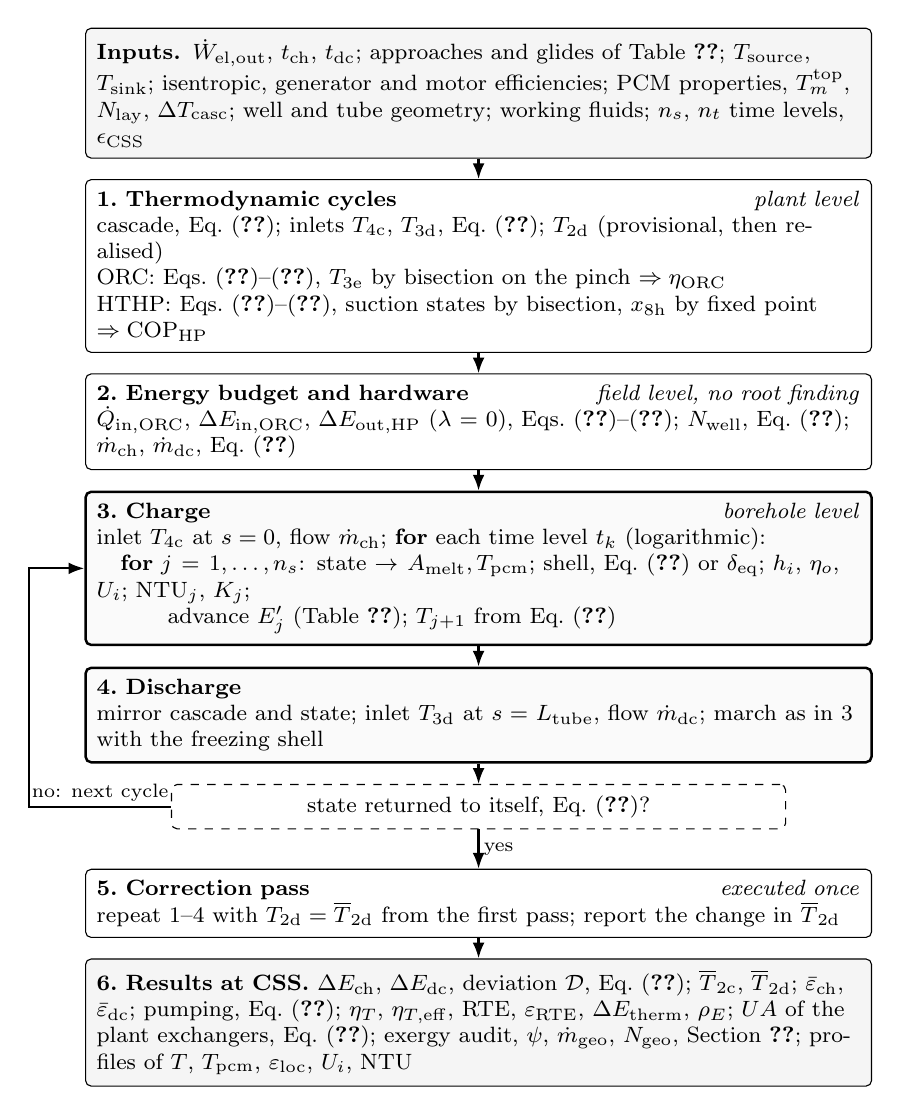
\begin{tikzpicture}[
  font=\footnotesize, node distance=2.6mm,
  blk/.style ={draw, rounded corners=2pt, inner sep=4pt, align=left,
               text width=0.80\linewidth},
  inp/.style ={blk, fill=black!4},
  mar/.style ={blk, line width=0.9pt, fill=black!2},
  tst/.style ={draw, dashed, rounded corners=2pt, inner sep=4pt, align=center,
               text width=0.62\linewidth},
  fl/.style  ={-{Latex[length=2mm]}, thick},
  lab/.style ={font=\scriptsize, inner sep=1.5pt}]

\node[inp] (in) {\textbf{Inputs.} $\dot W_\mathrm{el,out}$, $t_\mathrm{ch}$,
  $t_\mathrm{dc}$; approaches and glides of Table~\ref{tab:closure};
  $T_\mathrm{source}$, $T_\mathrm{sink}$; isentropic, generator and motor efficiencies; PCM
  properties, $T_m^\mathrm{top}$, $\Nlay$, $\Delta T_\mathrm{casc}$; well and
  tube geometry; working fluids; $n_s$, $n_t$ time levels,
  $\epsilon_\mathrm{CSS}$};

\node[blk, below=of in] (cyc) {\textbf{1.\ Thermodynamic cycles}
  \hfill\emph{plant level}\\
  cascade, Eq.~\eqref{eq:cascade}; inlets $T_\mathrm{4c}$, $T_\mathrm{3d}$,
  Eq.~\eqref{eq:inlets}; $T_\mathrm{2d}$ (provisional, then realised)\\
  ORC: Eqs.~\eqref{eq:orc-p}--\eqref{eq:T3e}, $T_\mathrm{3e}$ by bisection on
  the pinch $\Rightarrow\etaORC$\\
  HTHP: Eqs.~\eqref{eq:hp-p}--\eqref{eq:hp-T}, suction states by bisection,
  $x_\mathrm{8h}$ by fixed point $\Rightarrow\COP$};

\node[blk, below=of cyc] (bud) {\textbf{2.\ Energy budget and hardware}
  \hfill\emph{field level, no root finding}\\
  $\dot Q_\mathrm{in,ORC}$, $\Delta E_\mathrm{in,ORC}$, $\Delta
  E_\mathrm{out,HP}$ ($\lambda=0$), Eqs.~\eqref{eq:E-orc}--\eqref{eq:W-in};
  $\Nw$, Eq.~\eqref{eq:Nwell}; $\md_\mathrm{ch}$, $\md_\mathrm{dc}$,
  Eq.~\eqref{eq:mdot}};

\node[mar, below=of bud] (ch) {\textbf{3.\ Charge}\hfill\emph{borehole level}\\
  inlet $T_\mathrm{4c}$ at $s=0$, flow $\md_\mathrm{ch}$; \textbf{for} each
  time level $t_k$ (logarithmic):\\
  \hspace*{3mm}\textbf{for} $j=1,\ldots,n_s$: state $\to\Amelt,\Tpcm$;
  shell, Eq.~\eqref{eq:shell-choice} or $\delta_\mathrm{eq}$;
  $h_i$, $\etao$, $\Ui$; $\NTU_j$, $K_j$;\\
  \hspace*{9mm}advance $E'_j$ (Table~\ref{tab:alg-segment});
  $T_{j+1}$ from Eq.~\eqref{eq:T-march}};

\node[mar, below=of ch] (dc) {\textbf{4.\ Discharge}\\
  mirror cascade and state; inlet $T_\mathrm{3d}$ at $s=\Ltube$, flow
  $\md_\mathrm{dc}$; march as in 3 with the freezing shell};

\node[tst, below=of dc] (tst) {state returned to itself, Eq.~\eqref{eq:css-test}?};

\node[blk, below=5mm of tst] (cor) {\textbf{5.\ Correction pass}
  \hfill\emph{executed once}\\
  repeat 1--4 with $T_\mathrm{2d}=\overline{T}_\mathrm{2d}$ from the first
  pass; report the change in $\overline{T}_\mathrm{2d}$};

\node[inp, below=of cor] (out) {\textbf{6.\ Results at CSS.}
  $\Delta E_\mathrm{ch}$, $\Delta E_\mathrm{dc}$, deviation $\mathcal D$,
  Eq.~\eqref{eq:deviation}; $\overline{T}_\mathrm{2c}$,
  $\overline{T}_\mathrm{2d}$; $\bar\varepsilon_\mathrm{ch}$,
  $\bar\varepsilon_\mathrm{dc}$; pumping, Eq.~\eqref{eq:Wf}; $\eta_T$,
  $\eta_{T,\mathrm{eff}}$, RTE, $\varepsilon_\mathrm{RTE}$,
  $\Delta E_\mathrm{therm}$, $\rho_E$; $UA$ of the plant exchangers,
  Eq.~\eqref{eq:UA}; exergy audit, $\psi$, $\md_\mathrm{geo}$,
  $N_\mathrm{geo}$, Section~\ref{sec:exergy}; profiles of $T$, $\Tpcm$,
  $\eloc$, $\Ui$, $\NTU$};

\foreach \a/\b in {in/cyc,cyc/bud,bud/ch,ch/dc,dc/tst,cor/out}
  \draw[fl] (\a) -- (\b);
\draw[fl] (tst) -- node[lab,right] {yes} (cor);
\coordinate (L) at ($(ch.west)+(-7mm,0)$);
\draw[fl] (tst.west) -- (L |- tst.west)
  node[lab,midway,above] {no: next cycle} -- (L) -- (ch.west);
\end{tikzpicture}
\caption{Solution procedure. Blocks 1--2 are evaluated once per pass and
produce a fully specified field; blocks 3--4 are repeated until cyclic steady
state; block 5 is a second evaluation, not a loop.}
\label{fig:procedure}
\end{figure}

%-----------------------------------------------------------------------
\subsection{Simulation conditions}
\label{sec:conditions}
%-----------------------------------------------------------------------

The reference case is summarised in Table~\ref{tab:conditions}. The PCM
properties are consistent with the trimodal material of Saher \textit{et al.}\
\cite{Saher2024}: a top-layer melting temperature of \SI{150}{\celsius} and a
latent heat of \SI{380}{\kilo\joule\per\kilogram}; in the absence of reported
data, densities of \num{1550} and \SI{1450}{\kilogram\per\meter\cubed},
specific heats of \num{1280} and \SI{1800}{\joule\per\kilogram\per\kelvin}
and conductivities of \num{0.60} and \SI{0.45}{\watt\per\meter\per\kelvin}
are assumed for the solid and liquid, respectively. \chk{The cascade assumes a
family of PCMs of identical properties with melting points spanning
\SIrange{101}{150}{\celsius}; state this explicitly and discuss whether such a
family exists.} The wells are \SI{5000}{ft} (\SI{1524}{\meter}) deep with a
\SI{7}{in} (\SI{177.8}{\milli\meter}) bore, each containing two hairpins of
1\,$\tfrac14$\,in Schedule~80 tube with 24 fins per leg, which leaves
$\Vwell=\SI{27.68}{\meter\cubed}$ of PCM per well. The cell radius is
$r_\mathrm{cell}=\SI{44.45}{\milli\meter}$, so
$\delta_\mathrm{merge}=\SI{23.37}{\milli\meter}$, $\beta=2.109$,
$S=0.3467$ and $\delta_\mathrm{eq}=\SI{8.74}{\milli\meter}$.

\begin{table}[htbp]
\centering
\caption{Reference case.}
\label{tab:conditions}
\small
\resizebox{\linewidth}{!}{%
\begin{tabular}{@{}l l r@{}}
\toprule
 & quantity & value \\
\midrule
\multirow{4}{*}{Duty}
 & net electrical output $\dot W_\mathrm{el,out}$ & \SI{1}{\mega\watt} \\
 & charging / discharging window $t_\mathrm{ch}$, $t_\mathrm{dc}$ & \SI{10}{\hour} / \SI{10}{\hour} \\
 & HTHP source $T_\mathrm{source}$ / ORC sink $T_\mathrm{sink}$ & \SI{60}{\celsius} / \SI{20}{\celsius} \\
 & working fluid (ORC and HTHP) & cyclopentane \\
\midrule
\multirow{4}{*}{Machines}
 & isentropic: turbines $\eta_{s,t}$ / ORC pumps $\eta_{s,p}$ / compressors $\eta_{s,c}$ & 0.85 / 0.85 / 0.85 \\
 & generator $\eta_\mathrm{gen}$ / motor $\eta_\mathrm{mot}$ & 0.95 / 0.95 \\
 & ORC intermediate pressure & arithmetic mean \\
 & HTHP intermediate pressure & geometric mean \\
\midrule
\multirow{6}{*}{Approaches [K]}
 & $\Delta T_\mathrm{pinch,ORC}$ / $\Delta T_\mathrm{2D,3E}$ & 5 / 12 \\
 & $\Delta T_\mathrm{E,sink}$ / $\Delta T_\mathrm{sink,gl}$ & 5 / 0 \\
 & $\Delta T_\mathrm{2H,3C}$ / $\Delta T_\mathrm{sub}$ & 10 / 2 \\
 & $\Delta T_\mathrm{3A,4A}$ / $\Delta T_\mathrm{pinch,HPE}$ & 10 / 5 \\
 & $\Delta T_\mathrm{4C,M}$ / $\Delta T_\mathrm{M,1D}$ & 10 / 10 \\
 & glides $\Delta T_\mathrm{3C,2C}$ / $\Delta T_\mathrm{3D,2D}$ / $\Delta T_\mathrm{casc}$ & 55 / 55 / 55 \\
\midrule
\multirow{4}{*}{PCM}
 & $T_m^\mathrm{top}$ / $T_m^\mathrm{bot}$ / $\Nlay$ & \SI{150}{\celsius} / \SI{101.1}{\celsius} / 9 \\
 & $\hm$ & \SI{380}{\kilo\joule\per\kilogram} \\
 & $\rho_s$ / $\rho_l$; $c_{p,s}$ / $c_{p,l}$ & \SI{1550}{} / \SI{1450}{\kilogram\per\meter\cubed}; 1280 / \SI{1800}{\joule\per\kilogram\per\kelvin} \\
 & $k_s$ / $k_l$ & 0.60 / \SI{0.45}{\watt\per\meter\per\kelvin} \\
\midrule
\multirow{5}{*}{Geometry}
 & $\Lwell$ / $D_\mathrm{well}$ & \SI{1524}{\meter} / \SI{177.8}{\milli\meter} \\
 & hairpins per well $n_t$ & 2 \\
 & $r_i$ / $r_e$ / $k_\mathrm{wall}$ & \SI{16.23}{\milli\meter} / \SI{21.08}{\milli\meter} / \SI{45}{\watt\per\meter\per\kelvin} \\
 & $n_f$ / $L_f$ / $t_f$ & 24 / \SI{7.5}{\milli\meter} / \SI{1.5}{\milli\meter} \\
 & fouling $R''_{f,i}$ & \SI{e-3}{\meter\squared\kelvin\per\watt} \\
\midrule
\multirow{4}{*}{Geothermal source}
 & yield per producing well $\md_\mathrm{geo,well}$ & \SI{12.5}{\kilo\gram\per\second} \chk{provisional} \\
 & minimum reinjection temperature $T_\mathrm{reinj,min}$ & \SI{25}{\celsius} \chk{placeholder} \\
 & dead state $T_0$ & $T_\mathrm{sink}=\SI{20}{\celsius}$ \\
 & exergy convention & resource \\
\midrule
\multirow{3}{*}{Loop / numerics}
 & water pressure $p_\mathrm{w}$ & \SI{1}{\mega\pascal} \\
 & segments $n_s$ / time levels per half-cycle & 100 / 40 \chk{use 99 or 108} \\
 & first time level / CSS tolerance & \SI{1}{\second} / \SI{e-9}{\joule\per\meter} \\
\bottomrule
\end{tabular}}
\end{table}

The time levels are distributed logarithmically between \SI{1}{\second} and
the end of each window, $t_k=t_\mathrm{w}^{(k-1)/(n_t-1)}$ with $t_\mathrm{w}$
in seconds, so the last step of a \SI{10}{\hour} window is
\SI{8.5e3}{\second}. \chk{The warning raised by the code for $n_s=100$ and
$\Nlay=9$: a layer boundary falls inside a segment, which then carries a
melting temperature in error by up to one layer width (\SI{6.1}{\kelvin}).
Rerun with $n_s=99$ or $108$ for the paper, and report a grid-convergence
check in $n_s$ and $n_t$.}

\paragraph{Validity of H7 in the reference case} At the charging flow the
mean velocity in the tube is about \SI{1.25}{\meter\per\second}, so the water
transits the \SI{3048}{\meter} hairpin in about \SI{2.4e3}{\second}, or
\SI{7}{\percent} of the window. The heat capacity of the water in the tube is
\SI{26}{\percent} of the sensible capacity $C_l$ of the PCM it serves, but a
\SI{10}{\kelvin} swing of the water holds only \SI{1.2}{\percent} of the
latent inventory, so the unresolved start-up transient displaces little
energy although it occupies a noticeable fraction of the window.
\chk{Earlier drafts quote \SI{2264}{\second} and \SI{1.35}{\meter\per\second};
v0.11 and v0.12 give \SI{2438}{\second} and \SI{1.25}{\meter\per\second}.}

The yield of a geothermal producer is taken provisionally as
\SI{12.5}{\kilo\gram\per\second}, the value for a \SI{4500}{\meter},
\SI{206}{\celsius} repurposed well, which is deeper and hotter than the source
considered here; reported values for repurposed oil and gas wells range from
about \SIrange{1}{12.5}{\kilo\gram\per\second}. $N_\mathrm{geo}$ is inversely
proportional to this value and should be read as a scaling result.
\chk{add references for the per-well yield range and the \SI{4500}{\meter}
case study.}

The equations were implemented in Python with CoolProp \cite{CoolProp} for
fluid properties. \todo{Python/CoolProp versions; code availability
statement.}

%=======================================================================
\section{Results}
\label{sec:results}
%=======================================================================
% SKELETON. Subsections mirror the IHTC-18 paper. The numbers in
% Table~\ref{tab:ref-results} were produced with thums.py v0.13 at the case of
% Table~\ref{tab:conditions} (n_s = 100, which the code flags); regenerate
% them with the final numerics before use.

\subsection{Power-to-heat-to-power cycle analysis}
\label{sec:res-cycles}

\todo{$T$--$s$ diagram of both cycles at the reference case; table of state
points, pressures, $y$, $x_\mathrm{8h}$, $\varepsilon_\mathrm{R1}$,
$\varepsilon_\mathrm{R2}$, $\etaORC$, $\COP$, duties and flow rates.}
\todo{ORC evaporator composite curves showing the interior pinch at the onset
of boiling, with the hot-end rule overlaid: in the first pass $T_\mathrm{3e}$
falls from \SI{134.1}{\celsius} to \SI{95.1}{\celsius} and $\etaORC$ from 0.198
to 0.148 (v0.12, irreversible machines; the corresponding reversible values are
0.232 and 0.174).}
\todo{Cost of machine irreversibility: rerun with
$\eta_{s,t}=\eta_{s,p}=\eta_{s,c}=1$ (recovers $\etaORC=0.1738$, $\COP=2.759$)
and report the change in RTE; basis for a component-wise exergy balance.}
\todo{$UA$ of the four plant exchangers; the ORC condenser dominates.}

\subsection{Thermal analysis of the borehole regenerator at cyclic steady state}
\label{sec:res-BB}

\begin{table}[htbp]
\centering
\caption{Reference case at cyclic steady state (model v0.13, provisional).}
\label{tab:ref-results}
\small
\resizebox{\linewidth}{!}{%
\begin{tabular}{@{}l r l@{}}
\toprule
quantity & value & note \\
\midrule
$\COP$ / $\etaORC$ & 2.473 / 0.1487 & irreversible machines; corrected pass \\
$T_\mathrm{3e}$ & \SI{95.5}{\celsius} & pinch-limited (hot-end rule: \SI{136.5}{\celsius}) \\
$x_\mathrm{8h}$ / $y$ & 0.436 / 0.805 & \\
$\varepsilon_\mathrm{R1}$ / $\varepsilon_\mathrm{R2}$ & 0.205 / 0.120 & required, Eq.~\eqref{eq:eps-R} \\
HTHP suction superheat $T_\mathrm{1h}-T_\mathrm{13h}$ & \SI{14.3}{\kelvin} & \SI{26.5}{\kelvin} if isentropic \\
$\Nw$ & 15.62 & latent inventory, Eq.~\eqref{eq:Nwell} \\
$\md_\mathrm{ch}$ / $\md_\mathrm{dc}$ per hairpin & 0.965 / \SI{0.971}{\kilo\gram\per\second} & pinned by the glides, Eq.~\eqref{eq:mdot} \\
cycles to CSS & 73 & from a fully solid store \\
$\eta_\mathrm{storage}$ & 1.000000 & Eq.~\eqref{eq:css-unity} \\
deviation $\mathcal D$ & $+\SI{4.46}{\percent}$ & Eq.~\eqref{eq:deviation} \\
$\overline{T}_\mathrm{2d}$ / $\overline{T}_\mathrm{2c}$ & \SI{148.5}{\celsius} / \SI{102.5}{\celsius} & nominal 146.1 / 105.0 \\
$\bar\varepsilon_\mathrm{ch}$ / $\bar\varepsilon_\mathrm{dc}$ & 0.9704 / 0.0109 & cycled fraction 0.9595 \\
$\eta_T$ / $\eta_{T,\mathrm{eff}}$ & 0.1413 / 0.1365 & \\
RTE / $\varepsilon_\mathrm{RTE}$ & 0.3172 / 0.3044 & v0.11 (multipliers): 0.3003 \\
$\psi$ / $\psi_\mathrm{str}$ & 0.2356 / 0.2764 & Eq.~\eqref{eq:psi}, with pumping \\
$\md_\mathrm{geo}$ / $N_\mathrm{geo}$ & \SI{100.8}{\kilo\gram\per\second} / 8.07 & Eq.~\eqref{eq:mgeo}; $\md_\mathrm{geo,well}=\SI{12.5}{\kilo\gram\per\second}$ \\
$(\Nw+N_\mathrm{geo})/\dot W_\mathrm{el,out}$ & \SI{22.7}{\per\mega\watt} & storage plus geothermal wells \\
$\Delta E_\mathrm{therm}$ / $\Delta E_\mathrm{elec}$ per well & 4731 / \SI{646}{\kilo\watt\hour} & \\
$\rho_E$ & \SI{170.9}{\kilo\watt\hour\per\meter\cubed} & \\
pumping, charge / discharge & 34.9 / \SI{35.4}{\kilo\watt} & \SI{6.73}{\percent} of gross output \\
$UA$, four plant exchangers & \SI{2253}{\kilo\watt\per\kelvin} & ORC condenser 1135 \\
\bottomrule
\end{tabular}}
\end{table}

\chk{Grid sensitivity, v0.12 (not yet repeated on v0.13): with $n_s=99$ (layer boundaries on segment
boundaries) the deviation is $+\SI{4.44}{\percent}$ instead of
$+\SI{4.53}{\percent}$, $\bar\varepsilon_\mathrm{ch}$ is 0.980 instead of 0.972,
and the residual $\bar\varepsilon_\mathrm{dc}$ doubles, 0.025 instead of 0.012,
while RTE is unchanged to four figures. The residual melted fraction is the
diagnostic used to separate rate from inventory limitation, so the final runs
must use a layer-conforming grid and a convergence check.}

\todo{Profiles along the well at CSS (depth coordinate): $T$, $\Tpcm$ against
the $T_m$ staircase, $\eloc$ at several times in each half-cycle, $\Ui$ and
$\NTU$. Emphasise the sawtooth imposed by the cascade and where the PCM is
superheated or subcooled.}
\todo{Convergence to CSS: charged and discharged energy per cycle and state
drift versus cycle number.}
\todo{Decomposition of the energy per half-cycle into plateau and sensible
branches; peak superheat and subcooling.}
\todo{Resistance budget of $\Ui$ (convection, fouling, wall, PCM side) over a
half-cycle.}

\subsection{Exergy analysis}
\label{sec:res-exergy}

Table~\ref{tab:exergy} gives the exergy audit of the reference case over one
cycle. It is evaluated on the same basis as the round-trip efficiency: the
energy the field actually moved at cyclic steady state, with the borehole
parasitics charged as both an input and a destruction, so that $\psi$ and RTE
differ only in the charge made for the geothermal stream. Earlier drafts
evaluated it on the target duties and excluded the parasitics, which made the
two incomparable; the code was corrected to match this definition, not the
reverse. Three features stand out.

\begin{table}[htbp]
\centering
\caption{Exergy audit of the reference case over one cycle at CSS, resource
convention, $T_0=\SI{20}{\celsius}$ (model v0.13, provisional).}
\label{tab:exergy}
\small
\begin{tabular}{@{}l r r@{}}
\toprule
 & \si{\kilo\watt\hour} & share of $\sum I_j$ [\si{\percent}] \\
\midrule
\multicolumn{3}{@{}l}{\emph{inputs}}\\
electrical, $W_\mathrm{el,in}$ (incl.\ charge pumping) & 31813 & \\
geothermal, $\Ex_\mathrm{geo}$ (\SI{100.8}{\kilo\gram\per\second}) & 11019 & \\
\multicolumn{3}{@{}l}{\emph{outputs and loss}}\\
electrical, $W_\mathrm{el,out}$ & 10000 & \\
reinjected at \SI{50}{\celsius}, $\Ex_\mathrm{reinj}$ & 6326 & ($u_\mathrm{geo}=0.426$) \\
\midrule
\multicolumn{3}{@{}l}{\emph{destruction}}\\
HTHP condenser & 4584 & 17.4 \\
ORC evaporator & 3825 & 14.5 \\
HTHP throttle 7h$\to$8h & 3034 & 11.5 \\
HTHP compressor, high stage & 1915 & 7.3 \\
borehole field, Eq.~\eqref{eq:I-BB} & 1740 & 6.6 \\
HTHP motor & 1573 & 6.0 \\
ORC condenser & 1306 & 4.9 \\
HTHP evaporator & 1233 & 4.7 \\
HTHP compressor, low stage & 1222 & 4.6 \\
ORC turbine, low pressure & 1215 & 4.6 \\
HTHP throttle 9h$\to$4h & 1168 & 4.4 \\
ORC feed heater & 830 & 3.1 \\
borehole pumping & 703 & 2.7 \\
HTHP regenerator R2 & 671 & 2.5 \\
ORC generator & 550 & 2.1 \\
ORC turbine, high pressure & 511 & 1.9 \\
HTHP regenerator R1 & 320 & 1.2 \\
ORC pumps, mixer, flash separator & 12 & $<0.1$ \\
\midrule
$\sum I_j$ & 26415 & 100.0 \\
\bottomrule
\end{tabular}
\end{table}

First, heat transfer dominates. The five heat exchangers that carry the
process duty (HTHP condenser and evaporator, ORC evaporator and condenser, and
the borehole field) account for \SI{48.0}{\percent} of the destruction, the
compressors and turbines for \SI{18.5}{\percent}, and the motor and generator
for \SI{8.2}{\percent}. Second, the throttle between the condenser and the flash
separator destroys more exergy than either compressor stage, which indicates
that an expander in place of that valve is worth more than any plausible gain
in compressor efficiency. Third, the borehole field is responsible for only
\SI{6.8}{\percent} of the destruction; the case for the cascade and for tight
approach temperatures rests on the well count and the hardware rather than on
lost work \chk{$I_\mathrm{BB}$ is not yet independently verified}.

Pricing the geothermal stream lowers the headline efficiency from RTE $=0.317$
to $\psi=0.236$; under the stripped convention $\psi_\mathrm{str}=0.276$. The
geothermal flow required is \SI{100.8}{\kilo\gram\per\second}, i.e.\ 8.1
producers at the provisional yield, against 15.6 storage wells, and
\SI{57}{\percent} of the exergy lifted is reinjected.

\paragraph{Cooling of the source} $\Delta T_\mathrm{3A,4A}$ sets both the HTHP
evaporating temperature, and hence $\COP$, and the geothermal flow, which falls
much faster. Table~\ref{tab:dt3a4a} shows the consequence: the stripped
efficiency decreases monotonically, favouring the smallest cooling and the
largest geothermal flow, whereas the resource efficiency has an interior
maximum near \SI{20}{\kelvin}. At \SI{20}{\kelvin} the COP falls by
\SI{7.8}{\percent} relative to the reference case, while the geothermal flow
falls to \SI{47}{\percent} of its value: $N_\mathrm{geo}$ drops from
\num{8.07} to \num{3.80} and the whole field from \num{22.7} to
\SI{19.4}{\per\mega\watt}, for an RTE of \num{0.293}. The reference
value of \SI{10}{\kelvin} is therefore poorly placed, and the upper limit on
$\Delta T_\mathrm{3A,4A}$ is set by the formation constraint
$T_\mathrm{reinj,min}$, for which no measured value is yet available.

\begin{table}[htbp]
\centering
\caption{Effect of the cooling of the geothermal source. Every row is a
full cyclic-steady-state run on the basis of Eq.~\eqref{eq:psi}, with the
parasitics charged, so the rows are directly comparable with
Table~\ref{tab:ref-results}.}
\label{tab:dt3a4a}
\small
\begin{tabular}{@{}r r r r r r r@{}}
\toprule
$\Delta T_\mathrm{3A,4A}$ [K] & $\COP$ & RTE & $\md_\mathrm{geo}/\md_\mathrm{geo}^{(5\,\mathrm{K})}$ &
$u_\mathrm{geo}$ & $\psi_\mathrm{str}$ & $\psi$ \\
\midrule
5  & 2.582 & 0.3310 & 1.000 & 0.227 & 0.2833 & 0.1899 \\
10 & 2.473 & 0.3172 & 0.486 & 0.426 & 0.2764 & 0.2356 \\
15 & 2.373 & 0.3045 & 0.315 & 0.597 & 0.2698 & 0.2505 \\
20 & 2.280 & 0.2927 & 0.229 & 0.739 & 0.2634 & \textbf{0.2544} \\
25 & 2.194 & 0.2818 & 0.178 & 0.852 & 0.2571 & 0.2533 \\
30 & 2.114 & 0.2716 & 0.144 & 0.933 & 0.2511 & 0.2498 \\
\bottomrule
\end{tabular}
\end{table}

\subsection{Parametric assessment}
\label{sec:res-param}

\todo{Following the IHTC-18 paper: $\Nlay$ and the glide. Report RTE,
$\Nw$ (or $\mathcal D$ at fixed $\Nw$), $\bar\varepsilon_\mathrm{dc}$ and total
$UA$ on common axes. Expected interior optimum in $\Delta T_\mathrm{3D,2D}$
from the pinch, Eq.~\eqref{eq:pinch-necessary}, and in
$\Delta T_\mathrm{casc}$ subject to Eq.~\eqref{eq:span-bound}.}
\todo{$\mathcal D$ and $\bar\varepsilon_\mathrm{dc}$ versus $\Nw$ to separate
rate from inventory limitation.}
\todo{Carry $\psi$, $N_\mathrm{geo}$ and $(\Nw+N_\mathrm{geo})/\dot
W_\mathrm{el,out}$ in every parametric table; a study ranked on RTE alone
selects the free-source corner.}

\subsection{Limitations}
\label{sec:limitations}

\todo{Quantify, at least by estimate:}
(i)~H3 is at its limit at the reference case: the fronts of adjacent legs
meet over most of the well, so the residual solid in the corners between legs
is reached through a longer and narrower path than the annulus represents,
and the PCM-side resistance is understated;
(ii)~H9 neglects conduction between the two legs of a hairpin, which differ
by up to the cascade span at the wellhead;
(iii)~H6 neglects heat exchange with the formation, so the storage efficiency
is unity by construction and the store appears in the exergy audit only through
its internal destruction;
(iv)~the cycles have no pressure drop or heat loss in the exchangers and a
zero-approach ORC feed heater, and the isentropic efficiencies are constant;
(v)~the model has not been validated against experiment or against a
higher-fidelity (two-dimensional) conduction calculation. Items (i) and (ii)
are geometric questions about the cell boundary and would be settled together
by a two-dimensional conduction model of the real cross-section.

%=======================================================================
\section{Conclusions}
\label{sec:conclusions}
%=======================================================================
\todo{After Section~\ref{sec:results}.}

\section*{Acknowledgements}
\todo{Funding.}

%=======================================================================
\section*{Nomenclature}
%=======================================================================
\begingroup\small
\begin{longtable}{@{}p{0.16\linewidth}p{0.62\linewidth}p{0.16\linewidth}@{}}
$A$ & area; PCM cross-section per unit length & \si{\meter\squared}\\
$\Aav$ & PCM cross-section per hairpin per unit developed length & \si{\meter\squared}\\
$\Amelt$ & melted cross-section & \si{\meter\squared}\\
$C_s$, $C_l$ & sensible capacity per unit length & \si{\joule\per\meter\per\kelvin}\\
$c_p$ & specific heat & \si{\joule\per\kilogram\per\kelvin}\\
$D$ & diameter & \si{\meter}\\
$\mathcal D$ & deviation of delivered energy from target & --\\
$E'$ & PCM enthalpy per unit length & \si{\joule\per\meter}\\
$\Elat$, $\Eeq$ & latent capacity; equilibrium enthalpy per unit length & \si{\joule\per\meter}\\
$\Delta E$ & energy per cycle & \si{\joule}, \si{\kilo\watt\hour}\\
$f$ & Darcy friction factor & --\\
$h$ & specific enthalpy & \si{\joule\per\kilogram}\\
$h_i$, $h_e$ & internal, PCM-shell heat transfer coefficient & \si{\watt\per\meter\squared\per\kelvin}\\
$\hm$ & latent heat of fusion & \si{\joule\per\kilogram}\\
$K$ & segment conductance per unit length & \si{\watt\per\meter\per\kelvin}\\
$k$ & thermal conductivity & \si{\watt\per\meter\per\kelvin}\\
$L$ & length & \si{\meter}\\
$\md$ & mass flow rate per hairpin & \si{\kilogram\per\second}\\
$n_f$, $n_s$, $n_t$ & fins per leg, segments, hairpins per well & --\\
$\Nlay$, $\Nw$ & PCM layers, wells & --\\
$P_T$ & finned outer perimeter & \si{\meter}\\
$p$ & pressure & \si{\pascal}\\
$\dot Q$, $q'$ & heat rate; heat rate per unit length & \si{\watt}, \si{\watt\per\meter}\\
$R''_{f,i}$ & internal fouling resistance & \si{\meter\squared\kelvin\per\watt}\\
$r_i$, $r_e$, $r_\mathrm{cell}$ & tube inner, outer, and cell radius & \si{\meter}\\
$S$ & mean-to-surface shape factor & --\\
$s$ & developed coordinate; specific entropy & \si{\meter}; \si{\joule\per\kilogram\per\kelvin}\\
$T$ & temperature & \si{\kelvin}\\
$t$ & time; fin thickness & \si{\second}; \si{\meter}\\
$\Ui$ & overall coefficient on the inner area & \si{\watt\per\meter\squared\per\kelvin}\\
$UA$ & exchanger conductance & \si{\watt\per\kelvin}\\
$V$ & volume & \si{\meter\cubed}\\
$\dot W$, $W$ & power; work or electrical energy per cycle & \si{\watt}; \si{\kilo\watt\hour}\\
$\Ex$, $\Exd$ & exergy per cycle; exergy rate & \si{\kilo\watt\hour}; \si{\watt}\\
$I$ & exergy destruction per cycle & \si{\kilo\watt\hour}\\
$N_\mathrm{geo}$ & geothermal producing wells & --\\
$s_\mathrm{gen}$ & specific entropy generation & \si{\joule\per\kilogram\per\kelvin}\\
$T_0$ & dead-state temperature, $T_\mathrm{sink}$ & \si{\kelvin}\\
$u_\mathrm{geo}$ & fraction of the geothermal exergy used & --\\
$x_\mathrm{8h}$ & vapour fraction leaving the flash valve & --\\
$y$ & ORC reheat mass fraction & --\\[3pt]
\multicolumn{3}{@{}l}{\emph{Greek}}\\
$\beta$ & $r_\mathrm{cell}/r_e$ & --\\
$\Delta s$ & segment length & \si{\meter}\\
$\delta$ & shell thickness & \si{\meter}\\
$\varepsilon$ & melted fraction; effectiveness & --\\
$\eta$ & efficiency; $\eta_{s,t}$, $\eta_{s,p}$, $\eta_{s,c}$ isentropic efficiency of turbines, pumps, compressors & --\\
$\lambda$ & storage-loss allowance & --\\
$\rho$, $\rho_E$ & density; thermal energy density & \si{\kilogram\per\meter\cubed}; \si{\kilo\watt\hour\per\meter\cubed}\\
$\tau$ & relaxation time $C/K$ & \si{\second}\\
$\phi$ & fraction of ORC heat absorbed isothermally & --\\
$\psi$, $\psi_\mathrm{str}$ & exergetic efficiency, resource and stripped conventions & --\\[3pt]
\multicolumn{3}{@{}l}{\emph{Subscripts}}\\
\multicolumn{3}{@{}p{0.95\linewidth}@{}}{a source stream;
c, d secondary water during charging, discharging; ch, dc charging,
discharging; e ORC working fluid; geo geothermal; h HTHP refrigerant; l liquid;
m melting; reinj reinjected; s solid; w water; wf working fluid.}\\
\end{longtable}
\endgroup


\bibliographystyle{elsarticle-num}
\bibliography{p2h2p_refs}

\end{document}
